\chapter{无网格近似理论}
本章以再生核无网格法为例对伽辽金无网格法进行介绍,详细说明无网格形函数及其导数的构造过程,讨论无网格形函数的插值性。同时,介绍伽辽金无网格法在弹性力学问题和薄板问题上的应用。
\section{再生核无网格近似}
如图(\ref{nomeshpoint})所示的问题为例,无网格近似将求解域$\Omega$及其边界$\Gamma$离散为一系列无网格节点$\{\pmb{x}_I\}^{N\!P}_{I=1}$,
$N\!P$表示无网格节点数量。每个无网格节点$\pmb{x}_I$对应的形函数为$\Psi_I(\pmb{x})$,形函数影响域为$supp(\pmb{x}_I)$,
并要求影响域的覆盖域需包含求解域$\Omega$,即$\Omega\subseteq^{N\!P}_{I=1}supp(\pmb{x}_I)$。
考虑求解域$\Omega$内的一个变量$u(\pmb{x})$,其对应的无网格近似函数$u^h(\pmb{x})$可表示为:
\begin{equation}\label{ui}
\begin{split}
    u^h(\pmb{x})=\sum_{I=1}^{N\!P}\Psi_I(\pmb{x})d_{I}
\end{split}
\end{equation}
其中$d_{I}$表示与无网格节点$\pmb{x}_I$对应的节点系数。\par
\begin{figure}[H]
\centering
    
\includegraphics[scale=0.6]{Figure/nomesh/point.png}
    \caption{无网格离散示意图}\label{nomeshpoint}
\end{figure}\par
根据再生核近似理论\textsuperscript{\cite{liuReproducingKernelParticle1995}},无网格形函数可以假设为如下再生核形式:
\begin{equation}\label{shapefunction}
        \Psi_I(\pmb{x})=\sum_{I=1}^{N\!P}\pmb{p}^{[p]T}(\pmb{x}_I-\pmb{x})\pmb{c}(\pmb{x})\phi_s(\pmb{x}_I-\pmb{x})
\end{equation}
其中$\pmb{p}^{[p]}(\pmb{x})$为$p$阶的多项式基函数向量,其表达式为:
\begin{equation}
    \pmb{p}^{[p]}(\pmb{x})=\{1,\;x,\;y,\;\dotsb,\;x^iy^i,\;\dotsb,\;y^p\},\quad 0\le i+j \le p
\end{equation}
而$\phi_s(\pmb{x}_I-\pmb{x})$为附属于节点$\pmb{x}_I$的核函数,其影响域的大小由影响域尺寸$s$决定,核函数及其影响域的大小共同决定了无网格形函数的局部紧支性和光滑性。在二维情况下,核函数$\phi_s(\pmb{x}_I-\pmb{x})$的影响域通常为圆形域或者矩形域[]。本文的影响域形状均为矩形,矩形影响域的核函数可由下列公式计算得到:
\begin{equation}
    \phi_s(\pmb{x}_I-\pmb{x})=\varphi(r_x)\varphi(r_y),\quad r_x=\frac{\lvert x_I-x\rvert}{s_x},r_y=\frac{\lvert y_I-y \rvert}{s_y}
\end{equation}
其中$s_x$和$s_y$分别为$x$和$y$方向上影响域尺寸的大小,在均匀布置的节点下,计算时一般使得两个方向上的影响域大小相等即$s_x=s_y=s$。为保证紧支性和光滑性,$\varphi$通常取为阶次大于$p$的紧支函数。本文针对弹性力学问题,无网格基函数一般选择二阶或者三阶多项式基函数,核函数$\phi_s(\pmb{x}_I-\pmb{x})$取为三次样条函数:
\begin{equation}
    \varphi(r)=\frac{1}{3!}
\begin{cases}
    (2-2r)^3-4(1-2r)^3 &r\le \frac{1}{2}\\
    (2-2r)^3&\frac{1}{2}<r\le 1\\
    0&r>1
\end{cases}
\end{equation}\par
针对薄板和薄壳问题,无网格基函数一般选择三阶或四阶多项式基函数,核函数$\phi_s(\pmb{x}_I-\pmb{x})$取为五次样条函数:
\begin{equation}
        \varphi(r)=\frac{1}{5!}
\begin{cases}
        (3-3r)^5-6(2-3r)^5+15(1-3r)^5&r\le\frac{1}{3}\\
        (3-3r)^5-6(2-3r)^5&\frac{1}{3}<r\le\frac{2}{3}\\
        (3-3r)^5&\frac{2}{3}<r\le1\\
        0&r>1
\end{cases}
\end{equation}\par
最后,无网格形函数表达式(\ref{shapefunction})中$\pmb{c}$为待定系数向量,该待定系数通过满足下列一致性条件[]确定:
\begin{equation}\label{regeneration conditions}
    \sum_{I=1}^{N\!P}\Psi_I(\pmb{x})\pmb{p}(\pmb{x}_I-\pmb{x})=\pmb{0}
\end{equation}
将式(\ref{shapefunction})代入到式(\ref{regeneration conditions})中即可得到待定系数向量$\pmb{c}(\pmb{x})$的具体表达式:
\begin{equation}\label{c}
    \pmb{c}(\pmb{x})=\pmb{A}^{-1}(\pmb{x})\pmb{p}(\pmb{0})
\end{equation}
式中$\pmb{A}$为矩量矩阵:
\begin{equation}
        \pmb{A}(\pmb{x})=\sum_{I=1}^{N\!P}\pmb{p}^{[p]}(\pmb{x}_I-\pmb{x})\pmb{p}^{[p]T}(\pmb{x}_I-\pmb{x})\phi_s(\pmb{x}_I-\pmb{x})
\end{equation}\par
将(\ref{c})代入到式(\ref{shapefunction})中得到最终的再生核无网格形函数的表达式:
\begin{equation}\label{Pshapefunction}
\begin{split}
        \Psi_I(\pmb{x})=\pmb{p}^{[p]T}(\pmb{0})\pmb{A}^{-1}(\pmb{x})\pmb{p}^{[p]}(\pmb{x}_I-\pmb{x})\phi_s(\pmb{x}_I-\pmb{x})
\end{split}
\end{equation}\par
无网格形函数的一阶梯度可通过对无网格形函数$\Psi_I$求导得到:
\begin{equation}
    \Psi_{I,i}(\pmb{x})=\left ( \begin{aligned}
    &\pmb p_{,i}^{[p]T}(\pmb x_I-\pmb x)\pmb A^{-1}(\pmb x)\phi_s(\pmb x_I-\pmb x)\\
    +&\pmb p^{[p]T}(\pmb x_I-\pmb x)\pmb A_{,i}^{-1}\phi_s(\pmb x_I-\pmb x)\\
    +&\pmb p^{[p]T}(\pmb x_I-\pmb x)\pmb A^{-1}(\pmb x)\phi _{s,i}(\pmb x_I-\pmb x)\\
    \end{aligned} \right)
    \pmb p(\pmb 0)
\end{equation}
其中,下标“$,i$”表示对坐标$x_i$求导。进一步对上式再求一次导数可得形函数的二阶梯度为:
\begin{equation}
    \Psi_{I,ij}(\pmb{x})=\left( \begin{aligned}
    \pmb p_{,ij}^{[p]T}(\pmb x_I-\pmb x)\pmb A^{-1}(\pmb x)\phi_s(\pmb x_I-\pmb x)\\
    +\pmb p_{,i}^{[p]T}(\pmb x_I-\pmb x)\pmb A_{,j}^{-1}(\pmb x)\phi_s(\pmb x_I-\pmb x)\\
    +\pmb p_{,i}^{[p]T}(\pmb x_I-\pmb x)\pmb A^{-1}(\pmb x)\phi_{s,j}(\pmb x_I-\pmb x)\\
    +\pmb p^{[p]T}(\pmb x_I-\pmb x)\pmb A_{,ij}^{-1}(\pmb x)\phi_s(\pmb x_I-\pmb x)\\
    +\pmb p_{,j}^{[p]T}(\pmb x_I-\pmb x)\pmb A_{,i}^{-1}(\pmb x)\phi_s(\pmb x_I-\pmb x)\\
    +\pmb p^{[p]T}(\pmb x_I-\pmb x)\pmb A_{,i}^{-1}(\pmb x)\phi_{s,j}(\pmb x_I-\pmb x)\\
    +\pmb p^{[p]T}(\pmb x_I-\pmb x)\pmb A^{-1}(\pmb x)\phi_{s,ij}(\pmb x_I-\pmb x)\\
    +\pmb p_{,j}^{[p]T}(\pmb x_I-\pmb x)\pmb A^{-1}(\pmb x)\phi_{s,i}(\pmb x_I-\pmb x)\\
    +\pmb p^{[p]T}(\pmb x_I-\pmb x)\pmb A_{,j}^{-1}(\pmb x)\phi_{s,i}(\pmb x_I-\pmb x)\\
   \end{aligned} \right)
    \pmb p(\pmb 0)
\end{equation}
式中$\pmb A_{,i}^{-1}=-\pmb A^{-1}\pmb A_{,i}\pmb A^{-1},\pmb A_{,ij}^{-1}=-\pmb A^{-1}(\pmb A_{,ij}\pmb A^{-1}+\pmb A_{,i}\pmb A_{,j}^{-1}+\pmb A_{,j}\pmb A_{,i}^{-1})$。\par
\begin{figure}[H]
\centering
\begin{subcaptiongroup}
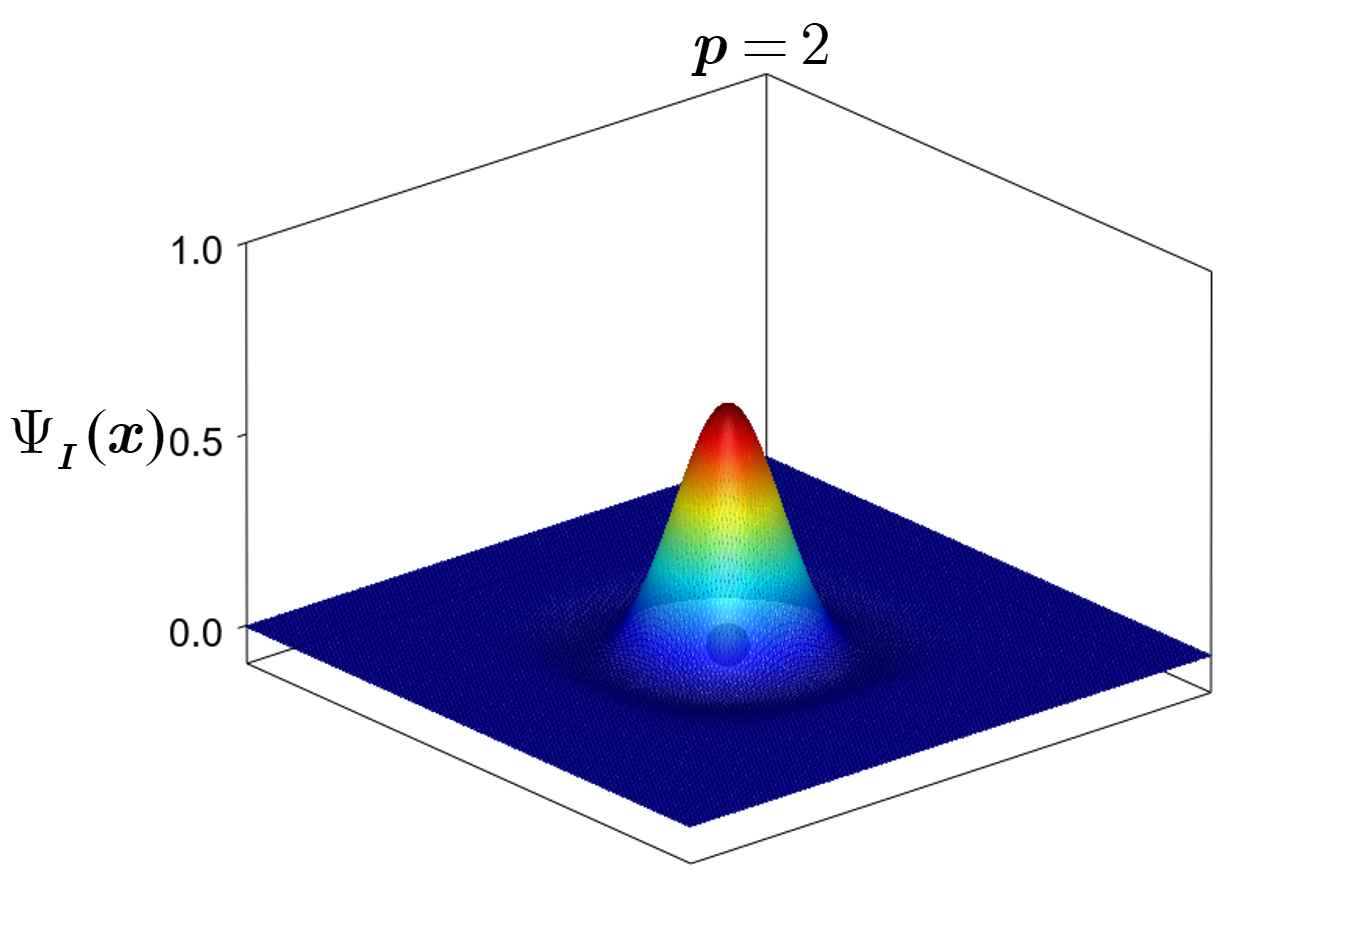
\includegraphics[width=0.3\textwidth]{figure/nomesh/QD41/1.png}
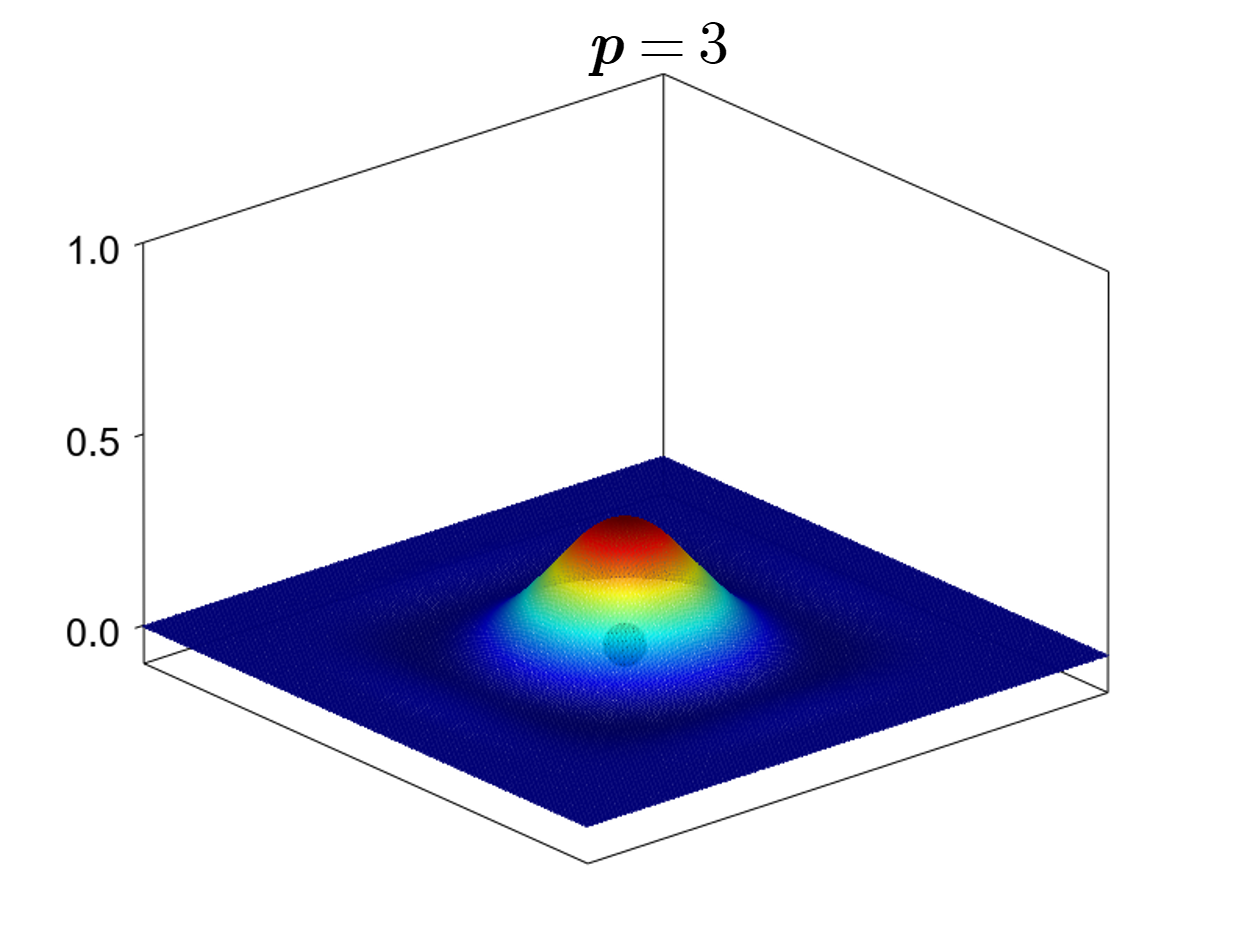
\includegraphics[width=0.3\textwidth]{figure/nomesh/C41/1.png}
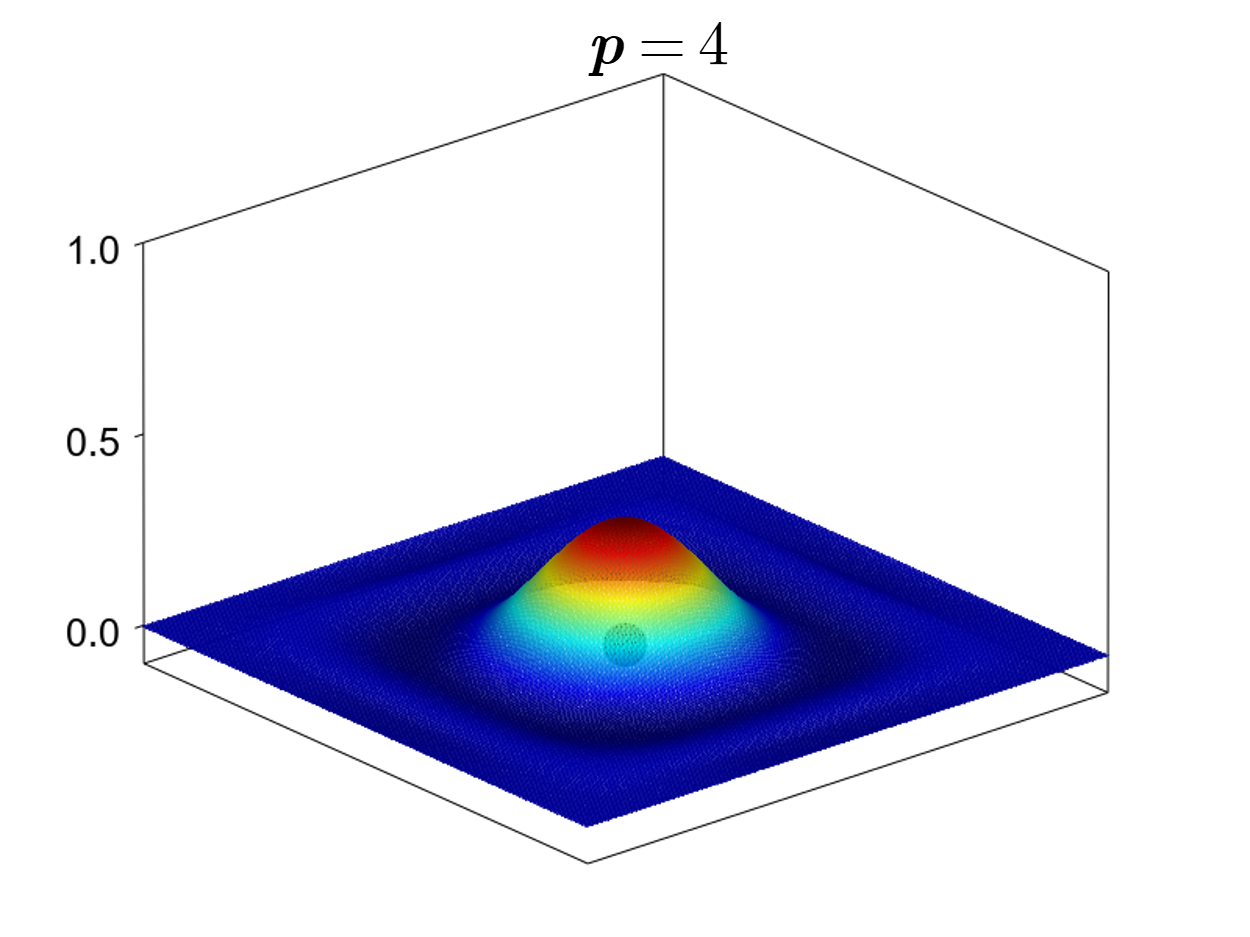
\includegraphics[width=0.3\textwidth]{figure/nomesh/QT41/1.png}
\end{subcaptiongroup}
 \begin{subcaptiongroup}
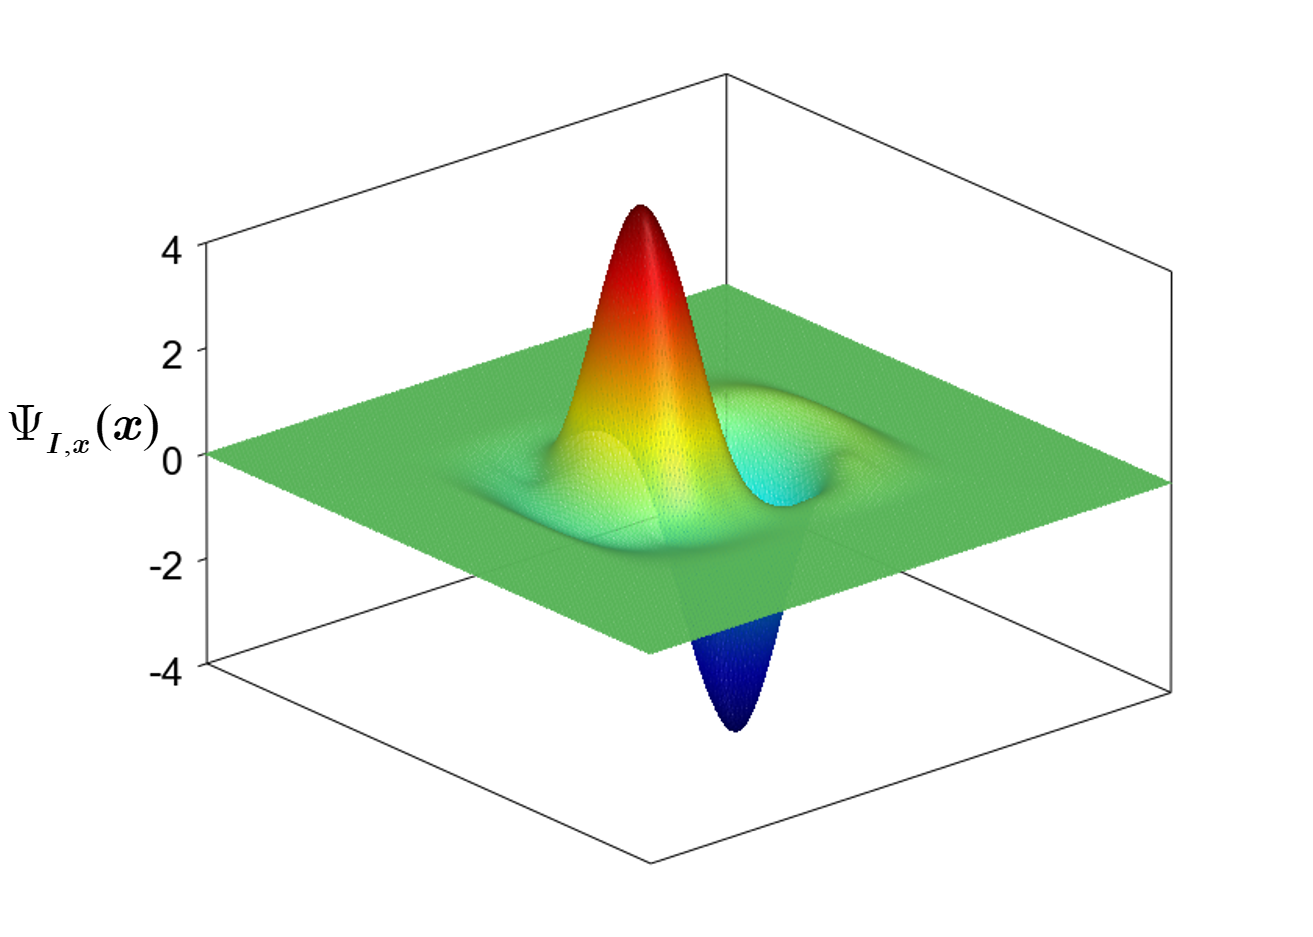
\includegraphics[width=0.3\textwidth]{figure/nomesh/QD41/2.png}
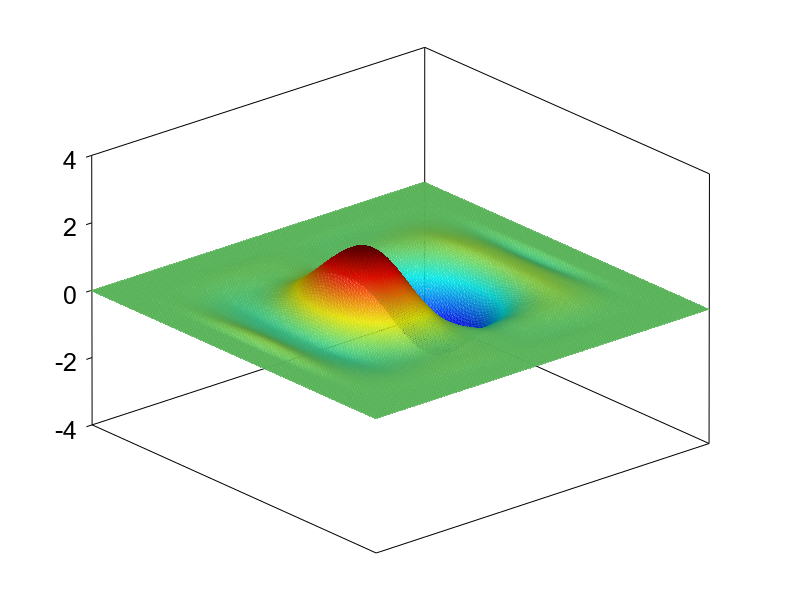
\includegraphics[width=0.3\textwidth]{figure/nomesh/C41/2.png}
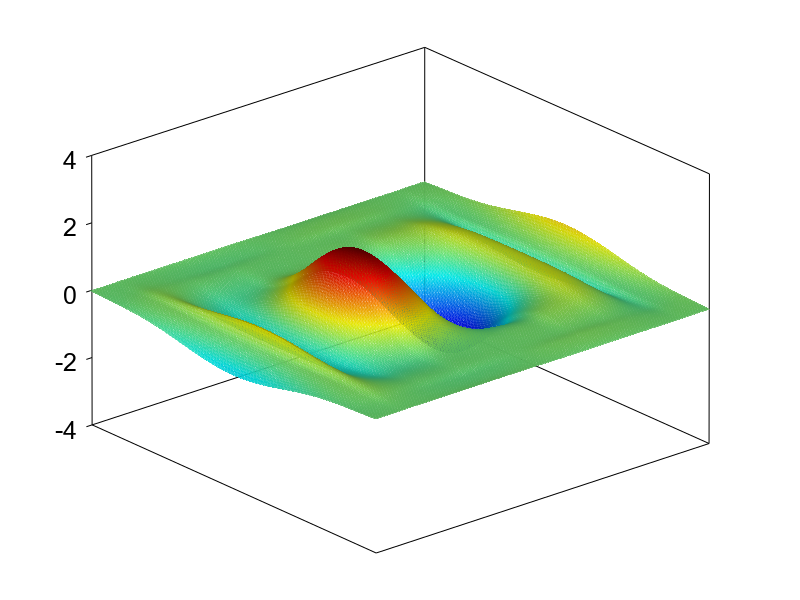
\includegraphics[width=0.3\textwidth]{figure/nomesh/QT41/2.png}
\end{subcaptiongroup}
\begin{subcaptiongroup}
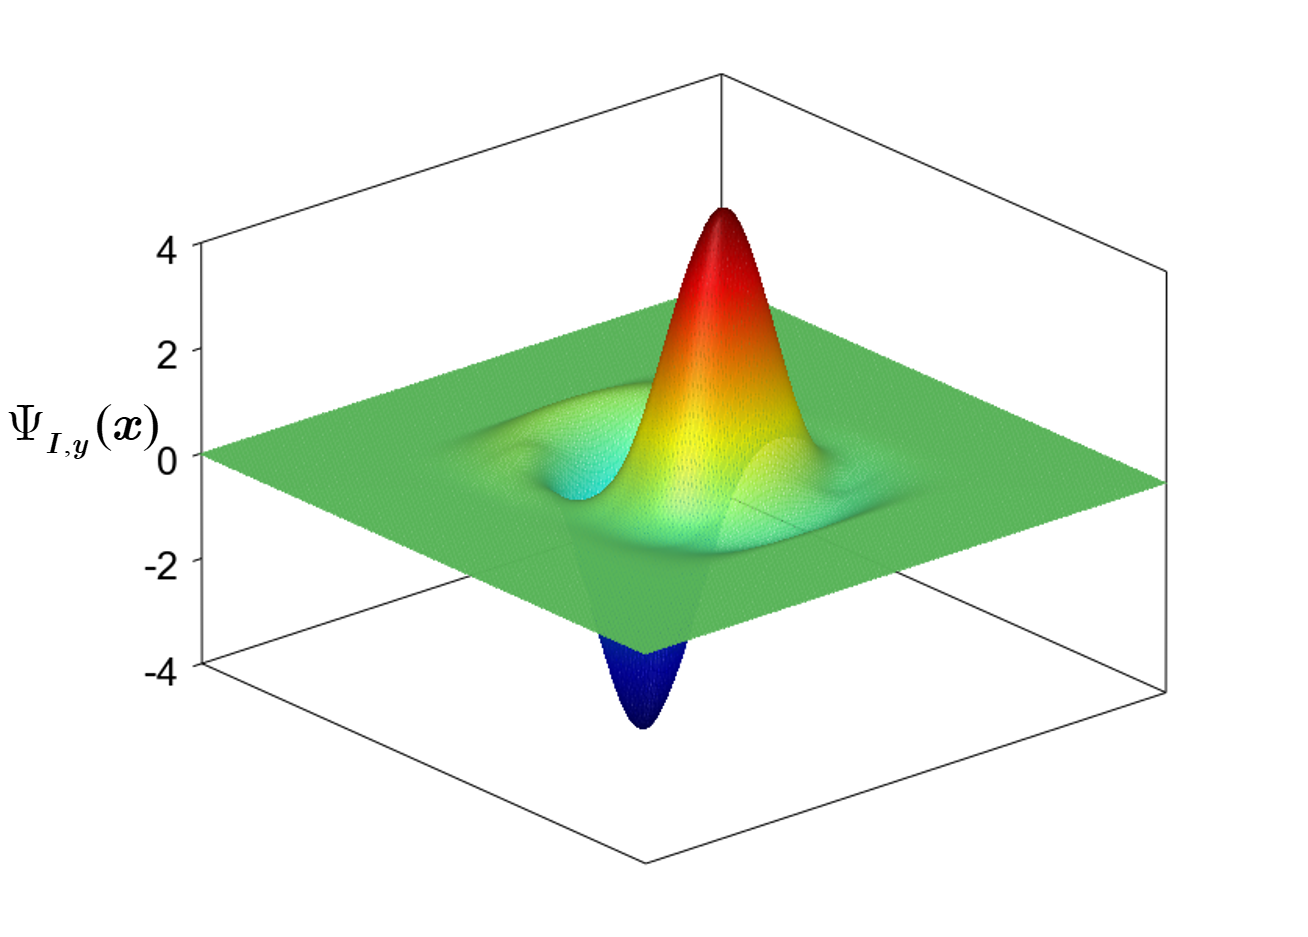
\includegraphics[width=0.3\textwidth]{figure/nomesh/QD41/3.png}
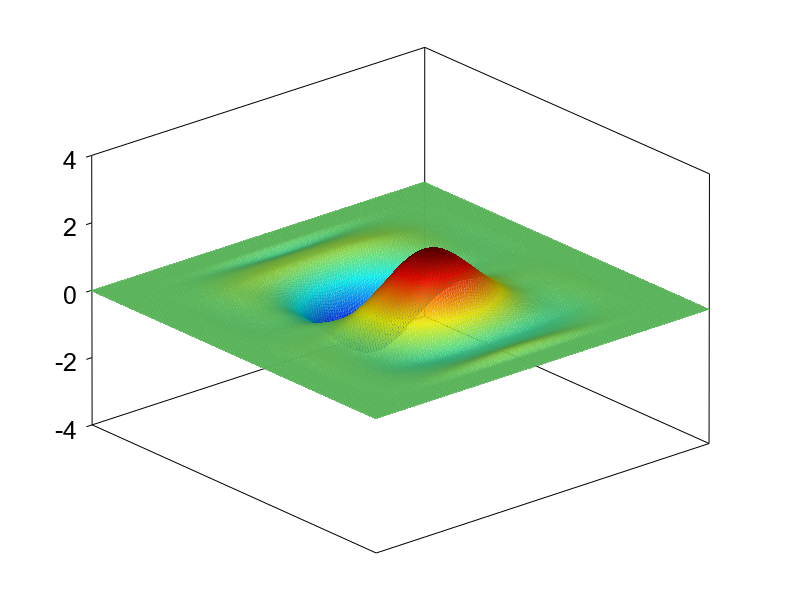
\includegraphics[width=0.3\textwidth]{figure/nomesh/C41/3.png}
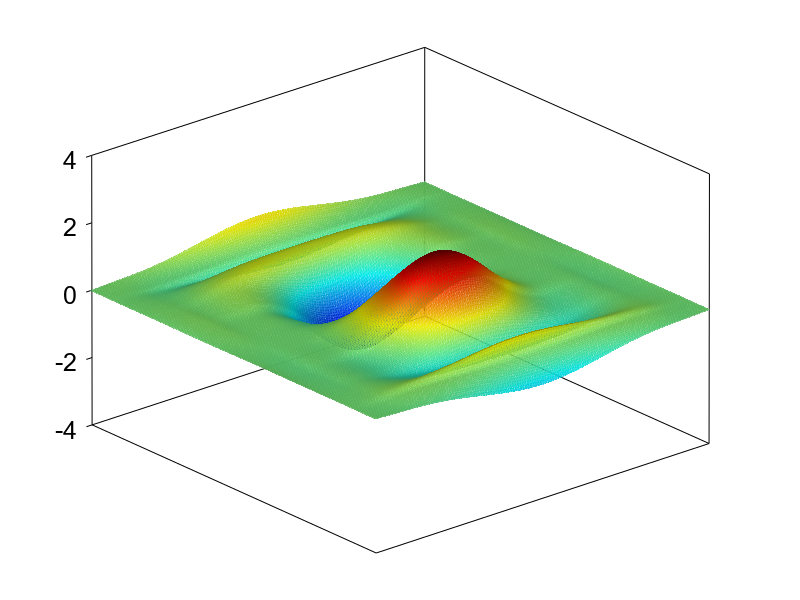
\includegraphics[width=0.3\textwidth]{figure/nomesh/QT41/3.png}
\end{subcaptiongroup}
\begin{subcaptiongroup}
    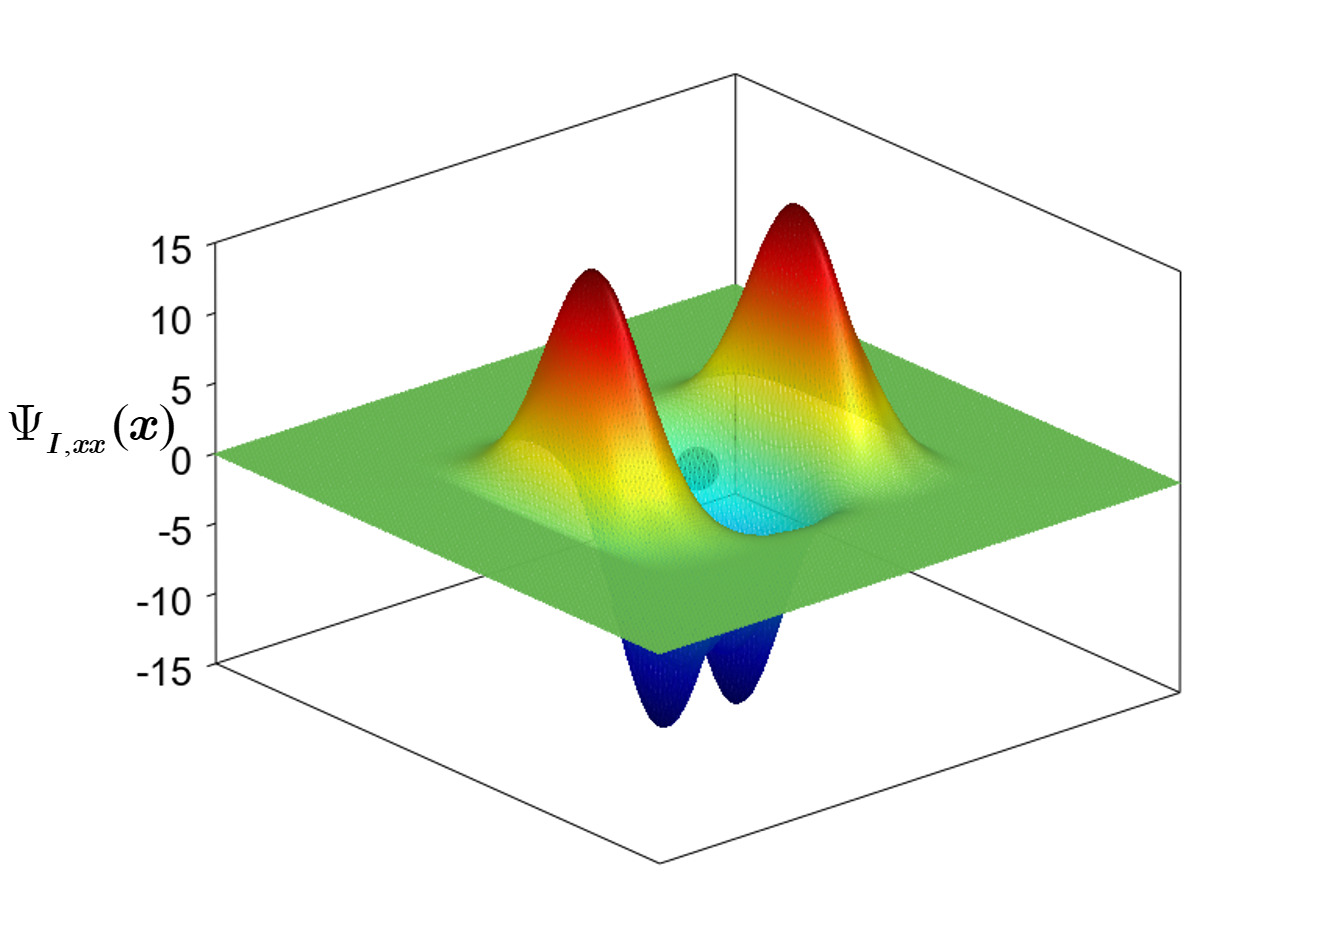
\includegraphics[width=0.3\textwidth]{figure/nomesh/QD41/4.png}
    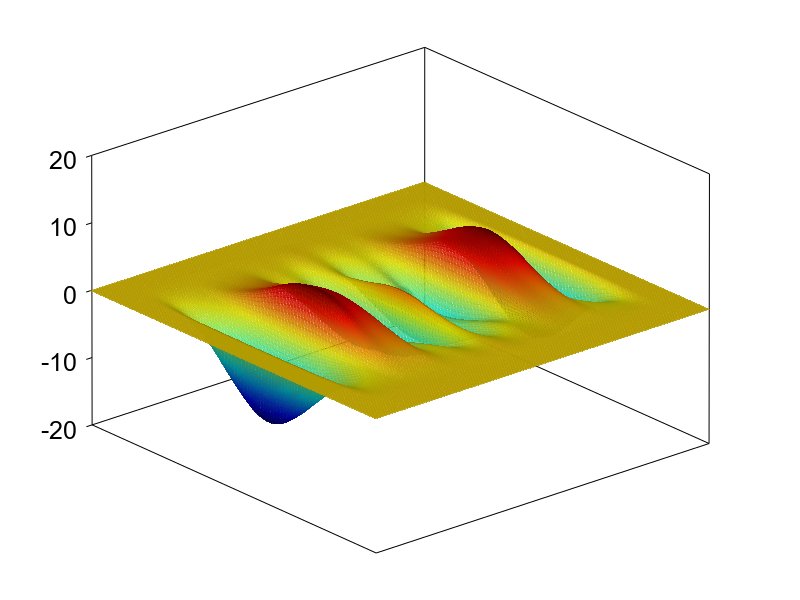
\includegraphics[width=0.3\textwidth]{figure/nomesh/C41/4.png}
    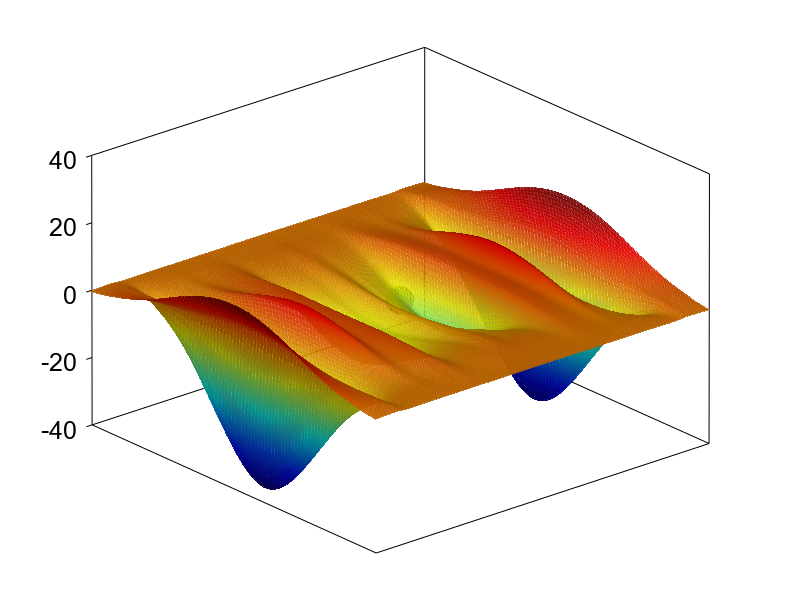
\includegraphics[width=0.3\textwidth]{figure/nomesh/QT41/4.png}
\end{subcaptiongroup}
\begin{subcaptiongroup}
    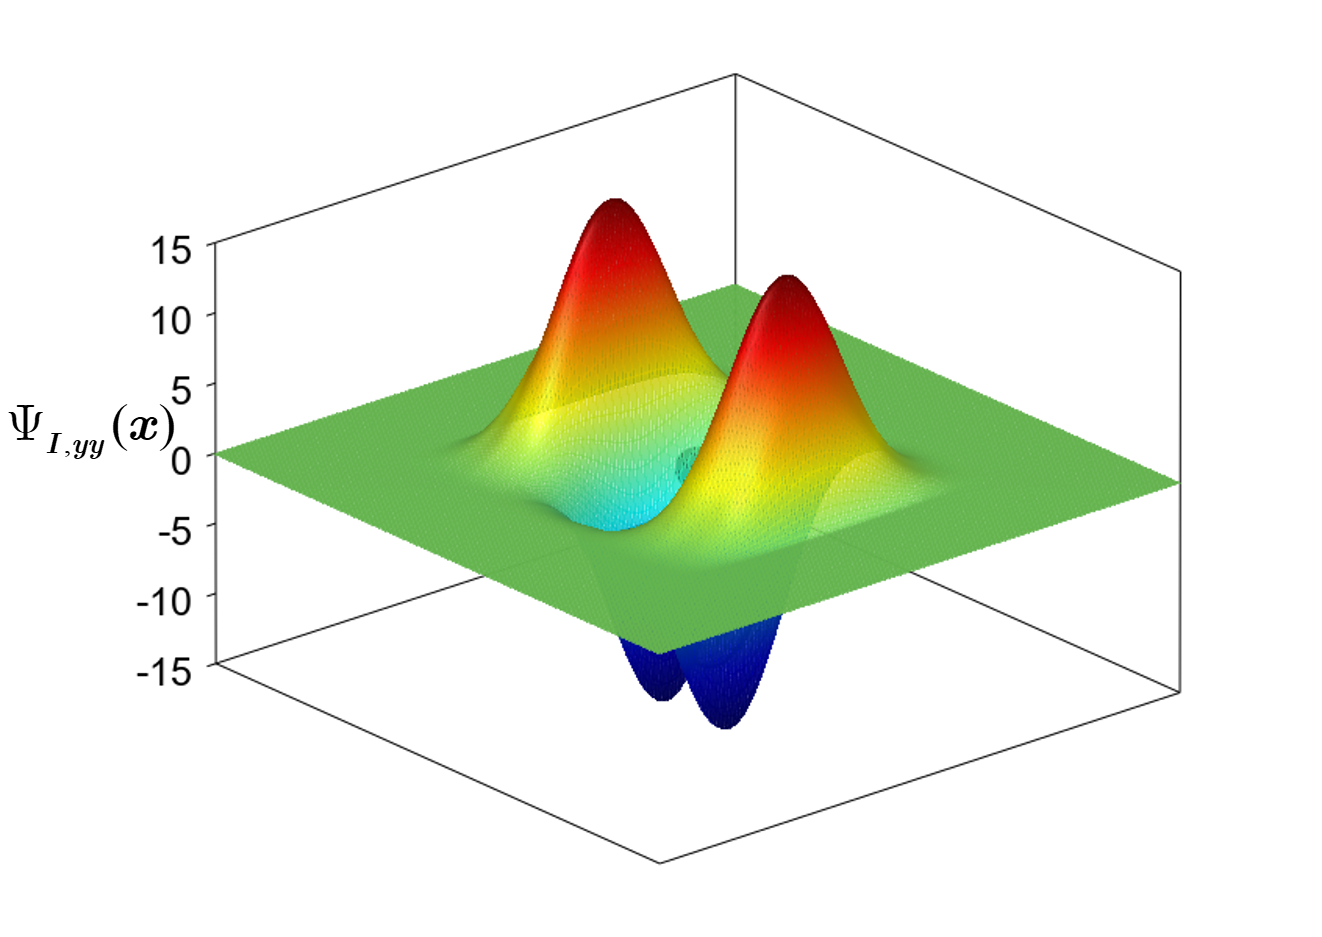
\includegraphics[width=0.3\textwidth]{figure/nomesh/QD41/5.png}
    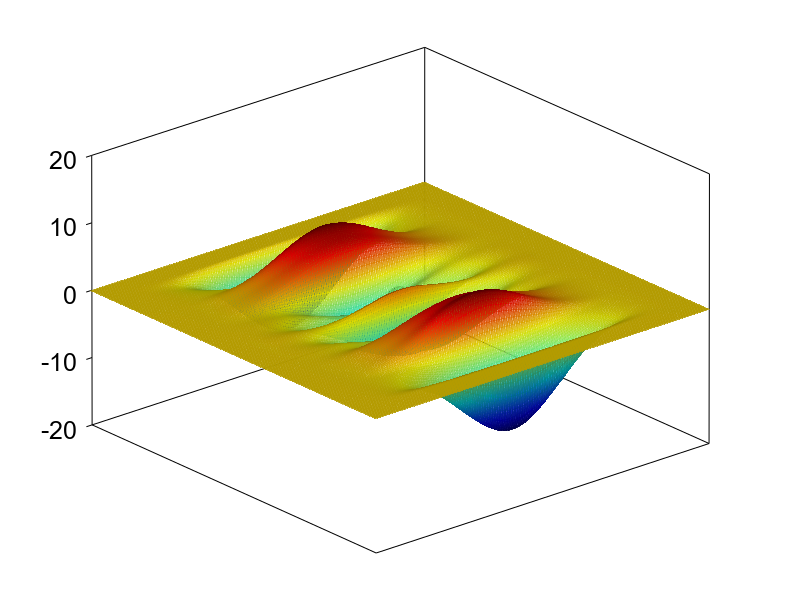
\includegraphics[width=0.3\textwidth]{figure/nomesh/C41/5.png}
    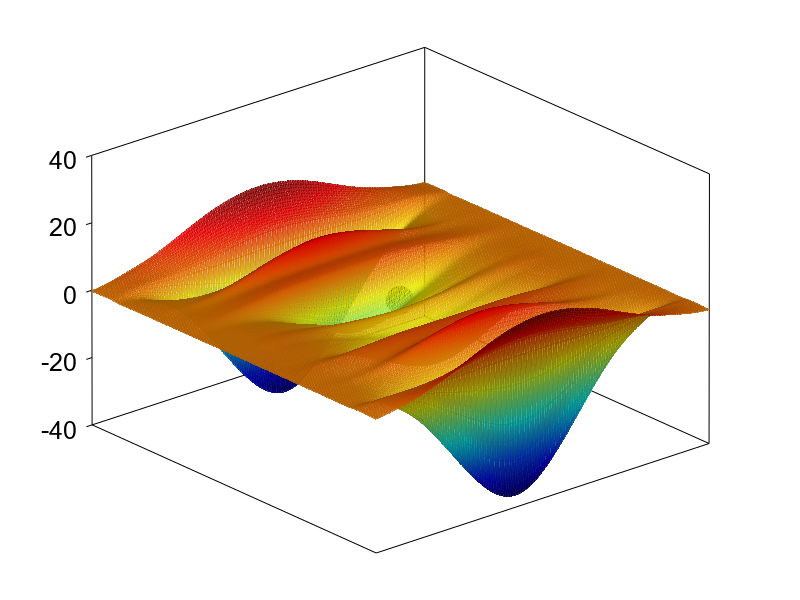
\includegraphics[width=0.3\textwidth]{figure/nomesh/QT41/5.png}
\end{subcaptiongroup}
\caption{二维内部节点无网格形函数及其一阶导数}\label{gradient1}
\end{figure}
\begin{figure}[H]
    \centering
    \begin{subcaptiongroup}
    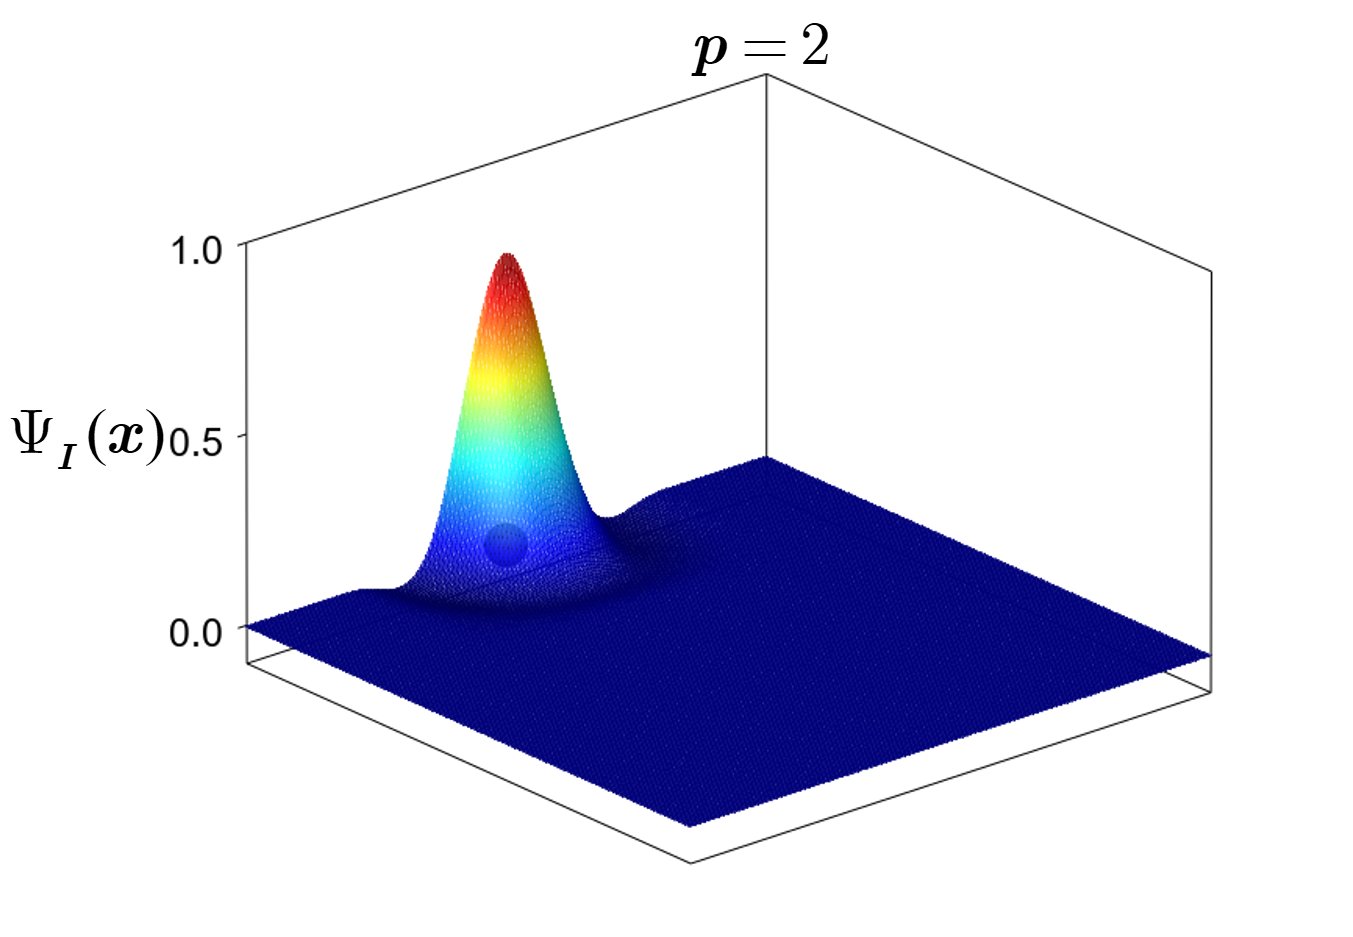
\includegraphics[width=0.3\textwidth]{figure/nomesh/QD77/1.png}
    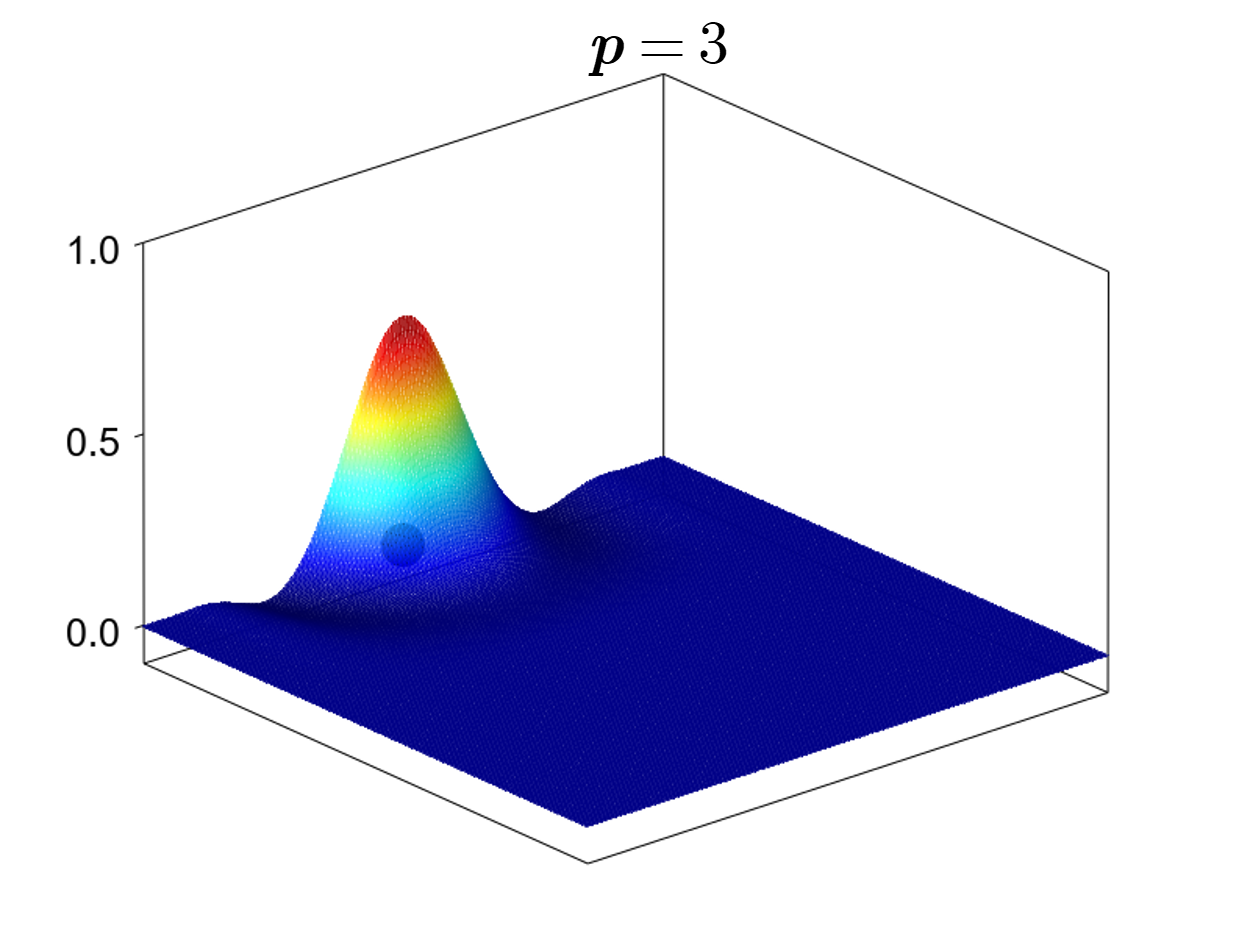
\includegraphics[width=0.3\textwidth]{figure/nomesh/C77/1.png}
    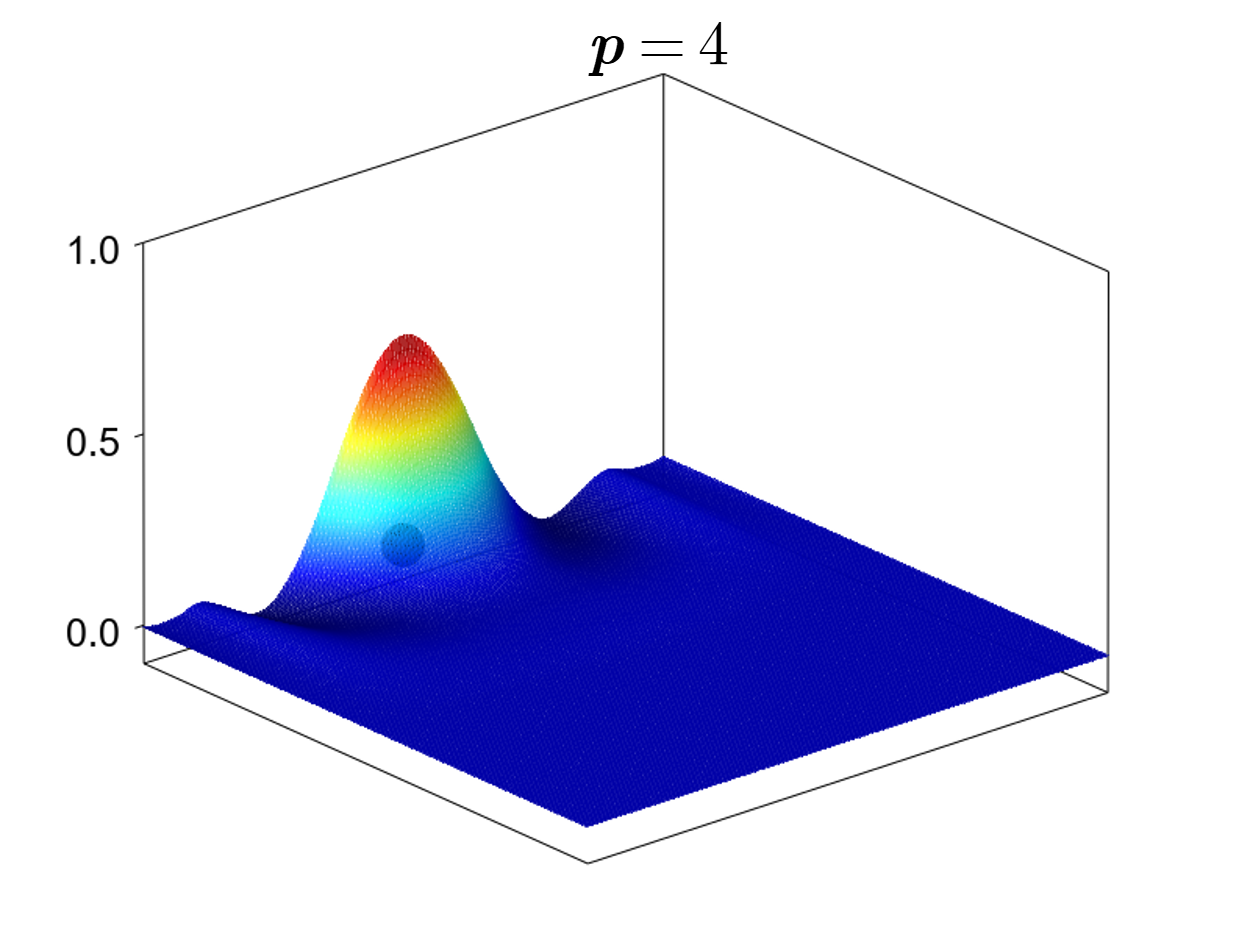
\includegraphics[width=0.3\textwidth]{figure/nomesh/QT77/1.png}
    \end{subcaptiongroup}
     \begin{subcaptiongroup}
    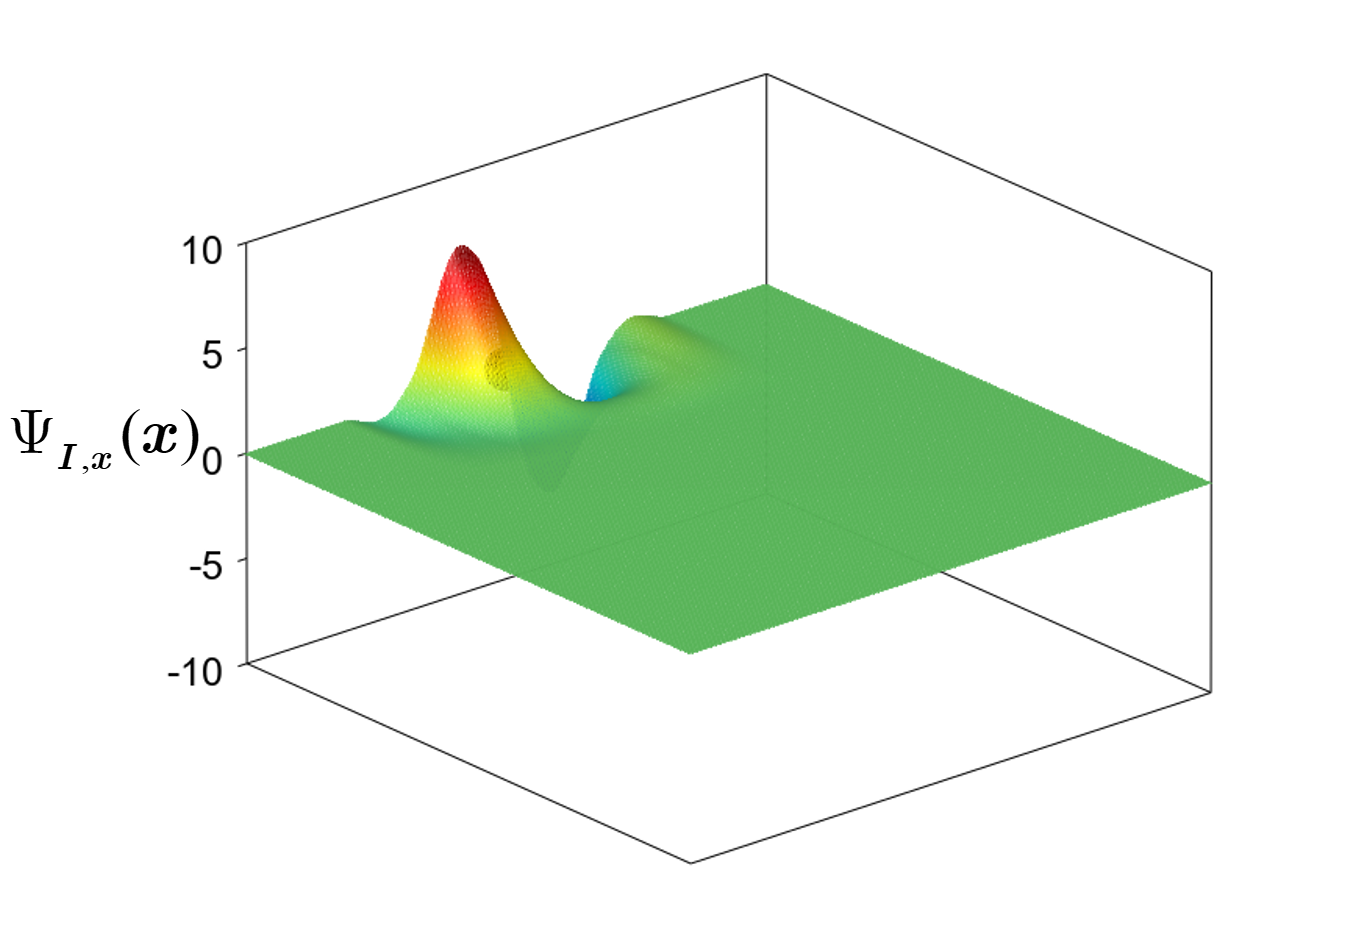
\includegraphics[width=0.3\textwidth]{figure/nomesh/QD77/2.png}
    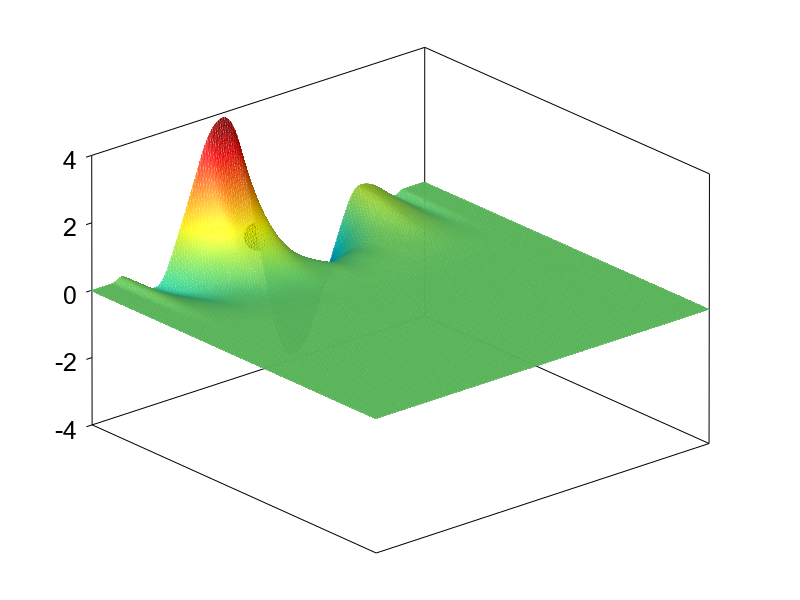
\includegraphics[width=0.3\textwidth]{figure/nomesh/C77/2.png}
    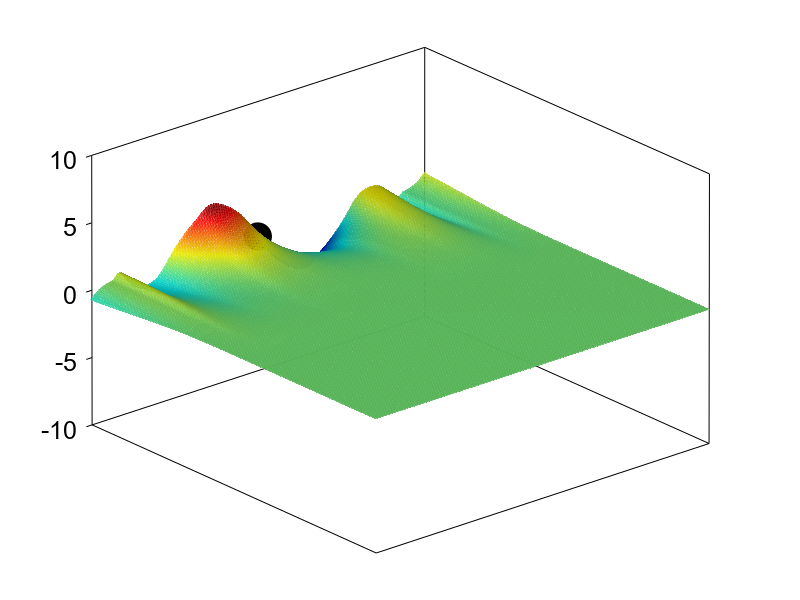
\includegraphics[width=0.3\textwidth]{figure/nomesh/QT77/2.png}
    \end{subcaptiongroup}
    \begin{subcaptiongroup}
    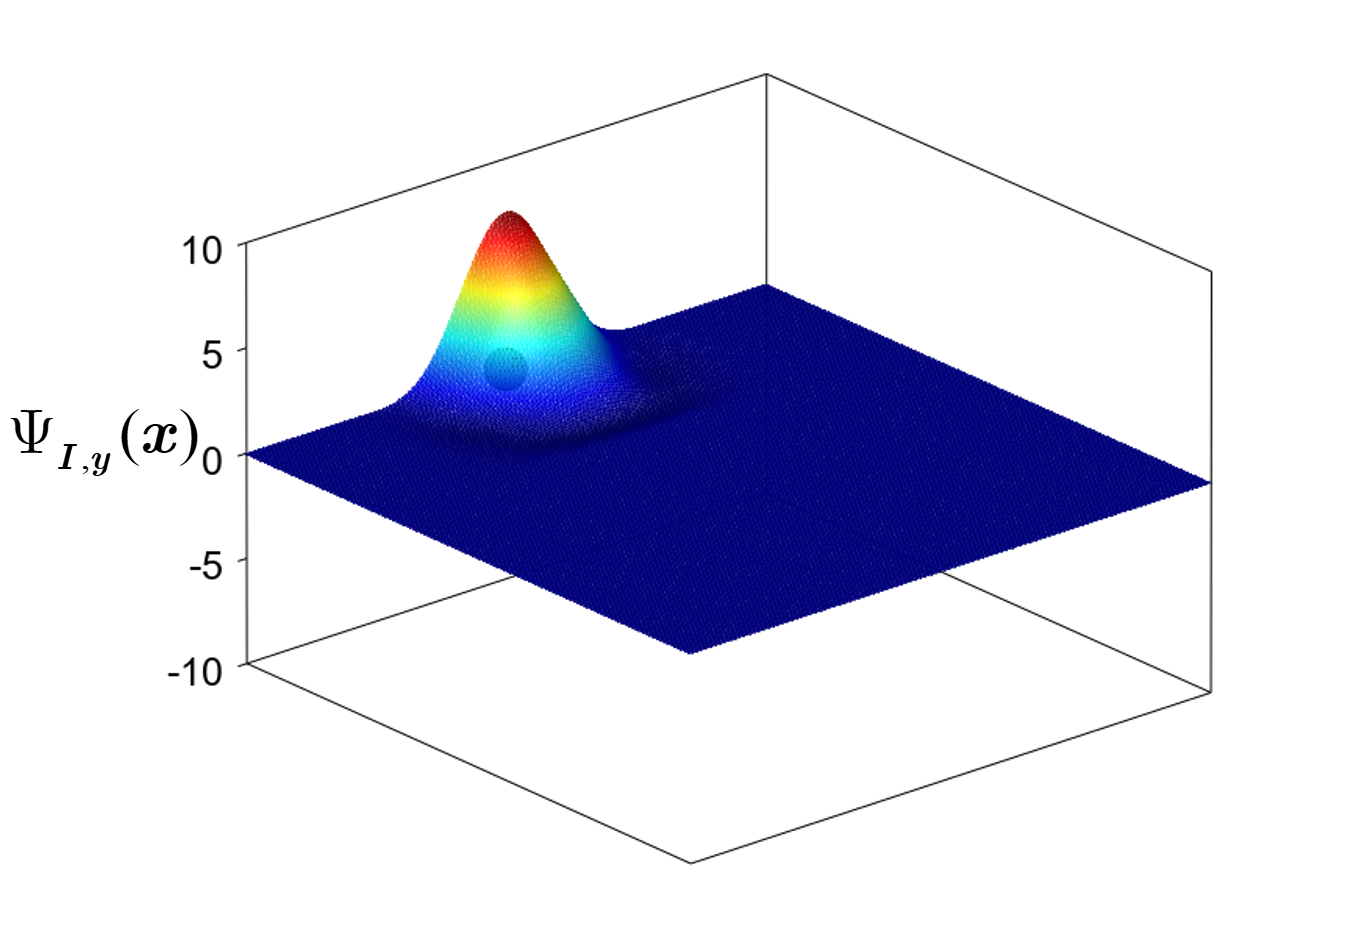
\includegraphics[width=0.3\textwidth]{figure/nomesh/QD77/3.png}
    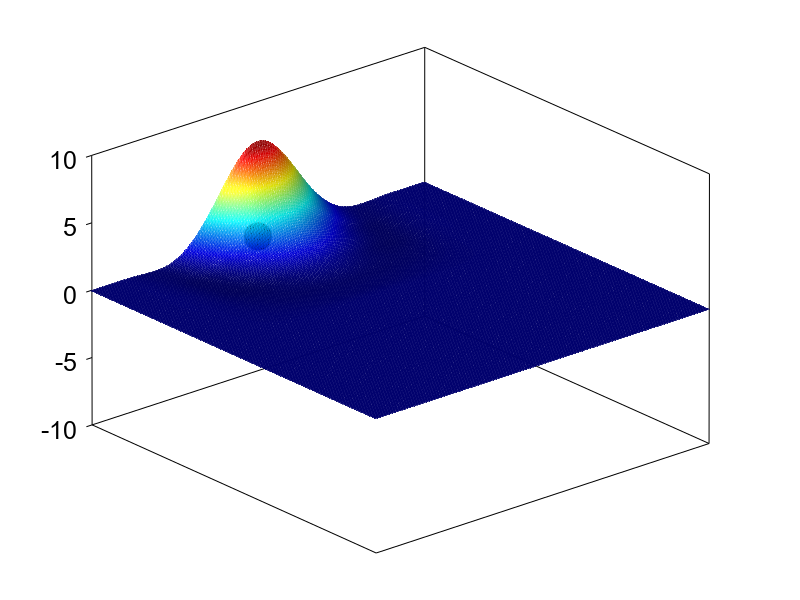
\includegraphics[width=0.3\textwidth]{figure/nomesh/C77/3.png}
    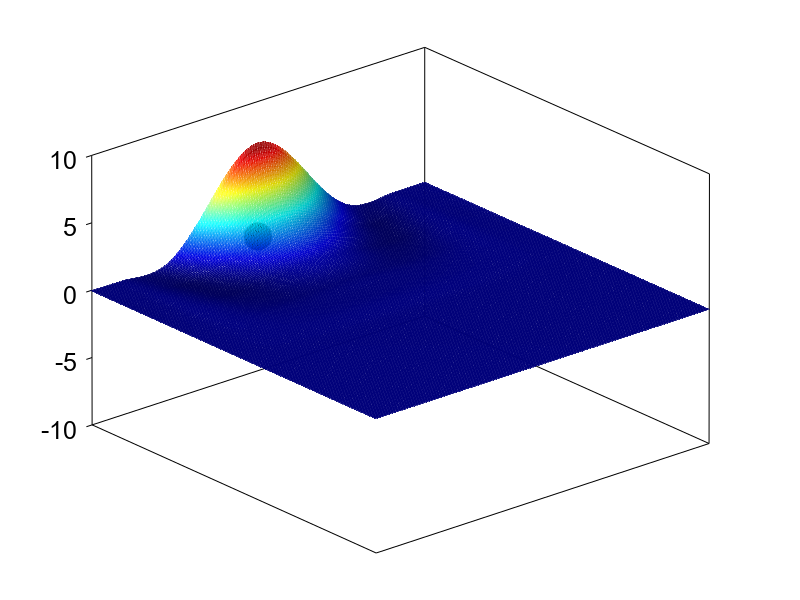
\includegraphics[width=0.3\textwidth]{figure/nomesh/QT77/3.png}
    \end{subcaptiongroup}
    \begin{subcaptiongroup}
        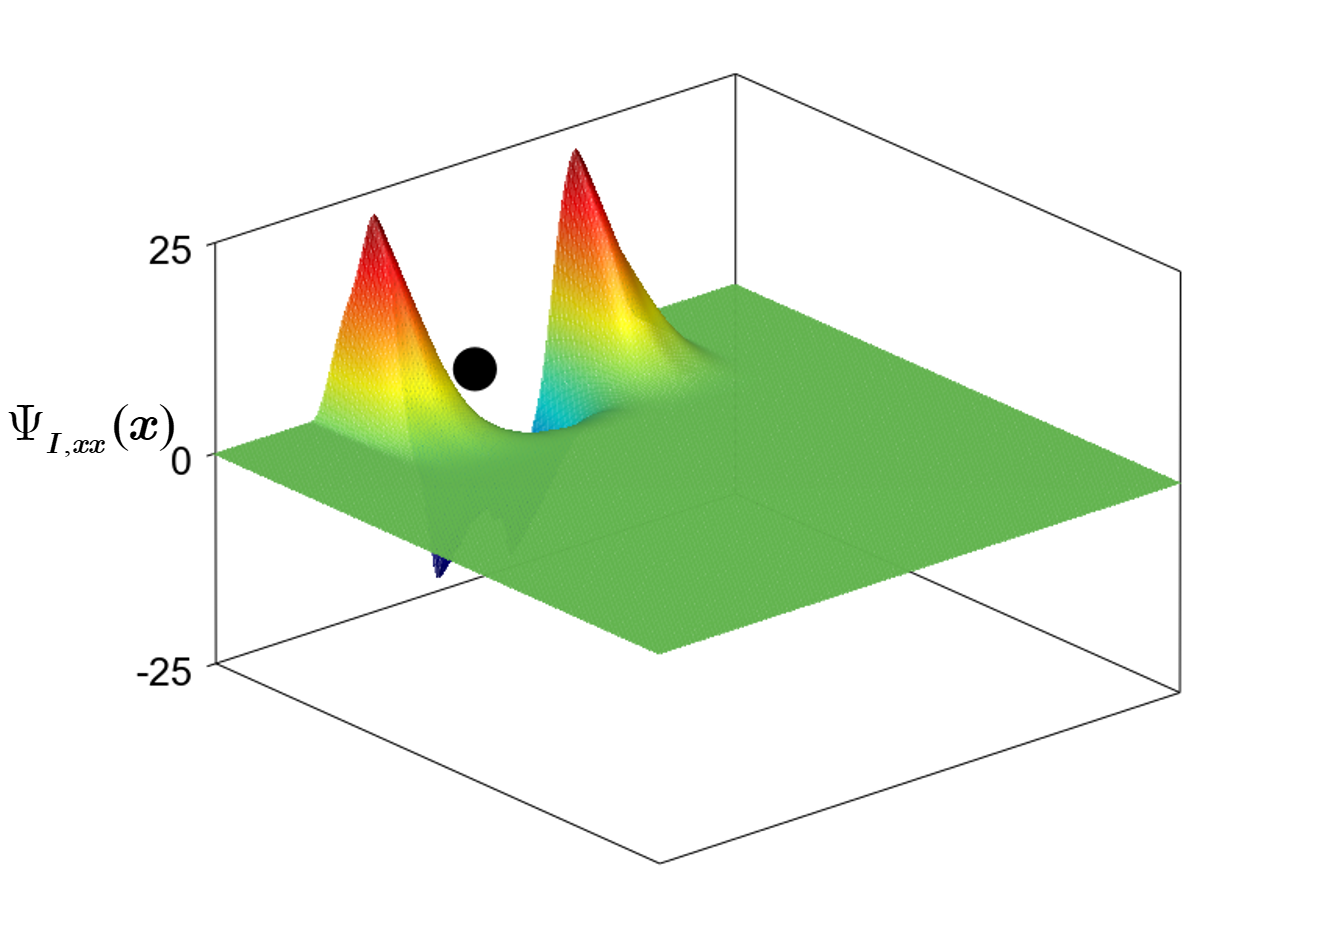
\includegraphics[width=0.3\textwidth]{figure/nomesh/QD77/4.png}
        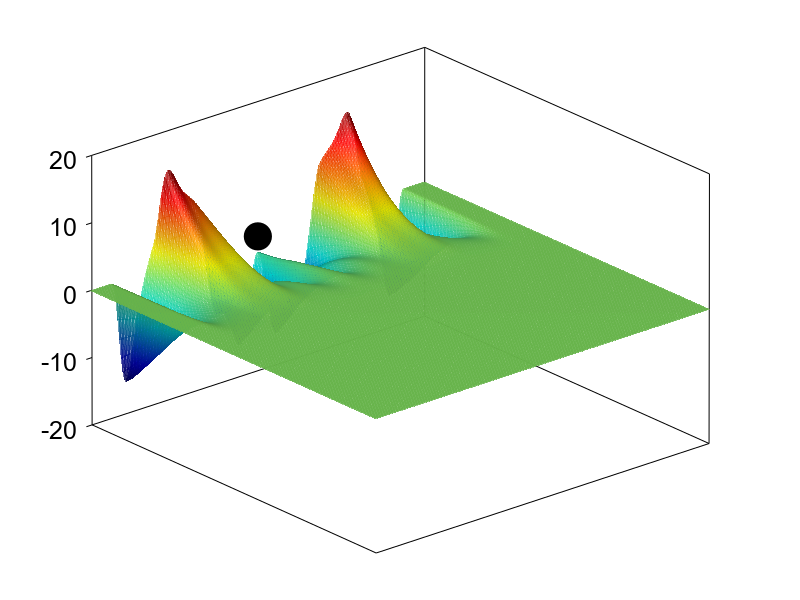
\includegraphics[width=0.3\textwidth]{figure/nomesh/C77/4.png}
        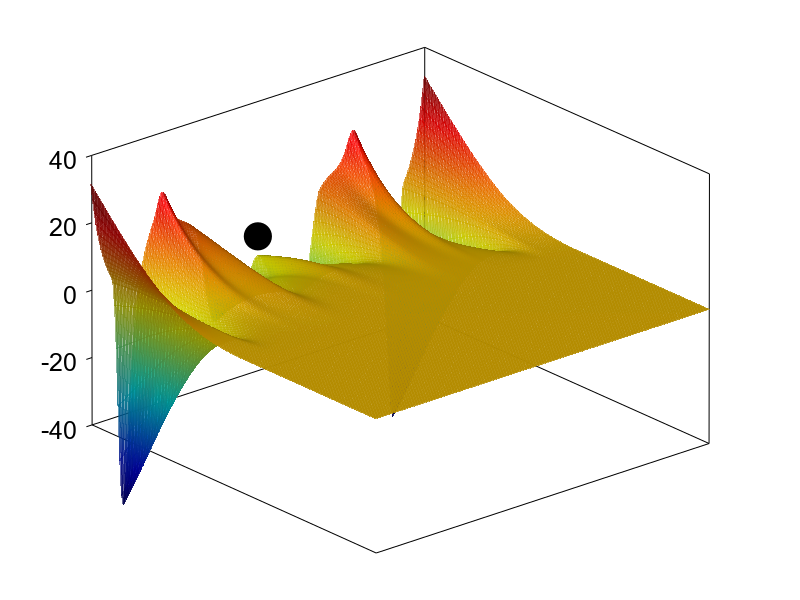
\includegraphics[width=0.3\textwidth]{figure/nomesh/QT77/4.png}
    \end{subcaptiongroup}
    \begin{subcaptiongroup}
        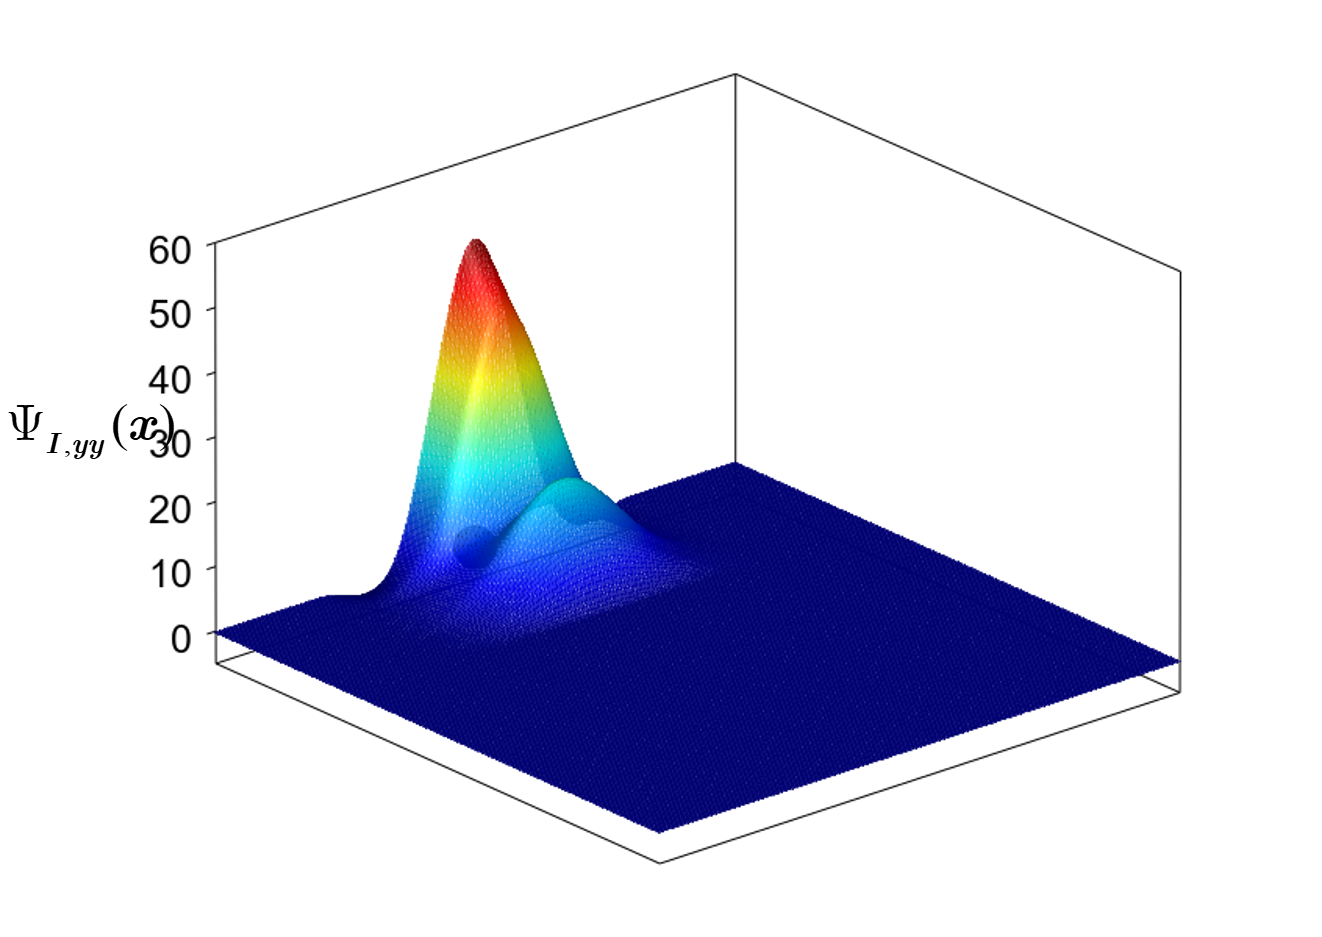
\includegraphics[width=0.3\textwidth]{figure/nomesh/QD77/5.png}
        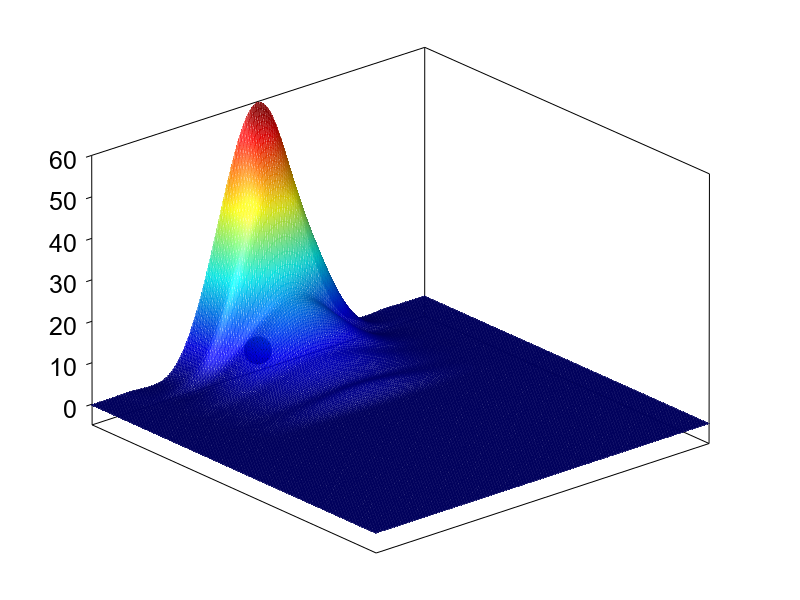
\includegraphics[width=0.3\textwidth]{figure/nomesh/C77/5.png}
        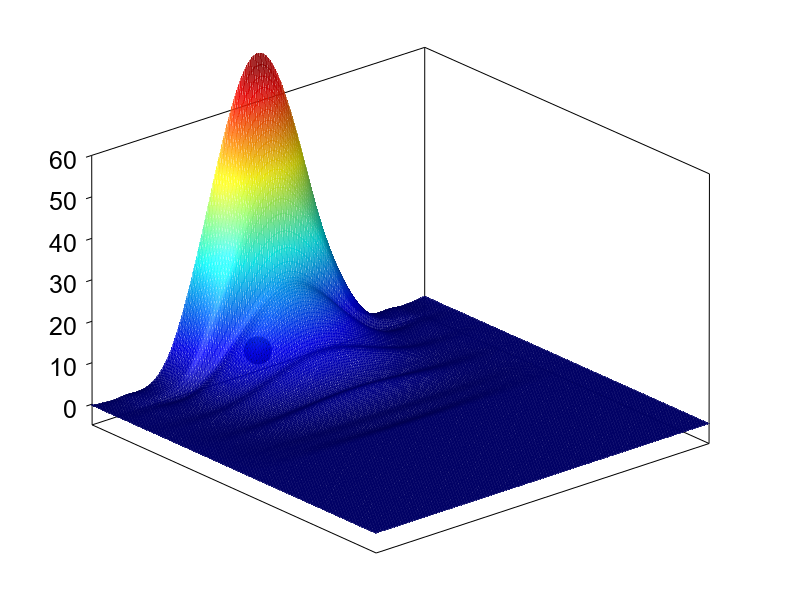
\includegraphics[width=0.3\textwidth]{figure/nomesh/QT77/5.png}
    \end{subcaptiongroup}
\caption{二维边界点处无网格形函数及其一阶导数}\label{gradient2}
\end{figure}
图(\ref{gradient1})、(\ref{gradient2})分别为内部节点和边界点处的无网格形函数及其导数图,从图中可知,无网格形函数具有全域高阶连续光滑的特点。但其无论是内部节点或边界点上的形函数在本点处均不具备插值性,即$\Psi_I(\pmb{x}_J)=\delta_{IJ}$。这将导致无网格法无法像有限元一样直接施加本质边界条件,需通过弱形式施加本质边界条件。
\newpage
\section{伽辽金无网格法}
\subsection{弹性力学问题}
不失为一般性,弹性力学问题的平衡微分方程为:
\begin{equation}\label{elasticity problems}
\begin{cases}
    \sigma_{ij,j}+b_i=0&\text{in}\;\Omega\\
    \sigma_{ij}n_j=t_i&\text{on}\;\Gamma^t\\
    u_i=g_i&\text{on}\;\Gamma^g
\end{cases}
\end{equation}
其中$\sigma_{ij}$为应力张量$\pmb \sigma$的分量,$u_i$为位移张量$\pmb{u}$的分量,$b_i$为体力张量$\pmb{b}$的分量。$\Gamma^t \text{、}\Gamma^g$分别表示自然和本质边界条件,并满足下列关系式:
\begin{equation}
\Gamma^t\cup \Gamma^g=\Gamma,\Gamma^t\cap \Gamma^g=\varnothing
\end{equation}
在自然和本质边界上具有给定的面力$\pmb{t}$和位移$\pmb{g}$,其分量分别为$t_i$和$g_i$。$n_i$为$\Gamma^{t}$上外法向量$\pmb{n}$的分量。\par
对于线弹性各向同性材料,其本构关系为:
\begin{equation}\label{constitutive relation}
    \sigma_{ij}=C_{ijkl}\varepsilon_{kl}
\end{equation}
其中$C_{ijkl}$为四阶弹性张量,$\varepsilon_{ij}$为应变张量的分量,根据小变形假设,应变$\varepsilon_{ij}$为:
\begin{equation}\label{CH2-strain}
    \varepsilon_{ij}=\frac{1}{2}(u_{i,j}+u_{j,i})
\end{equation} \par
根据最小势能原理,强形式(\ref{elasticity problems})所对应的势能泛函表达式为:
\begin{equation}\label{elasticity potential functional}
\begin{split}
    \Pi(\pmb{u})=\frac{1}{2}\int_{\Omega}\varepsilon_{ij}C_{ijkl}\varepsilon_{kl}d\Omega-\int_{\Omega}u_ib_id\Omega-\int_{\Gamma^t}u_it_id\Gamma
\end{split}
\end{equation}
对式(\ref{elasticity potential functional})进行变分可以得到式(\ref{elasticity problems})的等效积分弱形式:
\begin{equation}\label{elasticity weak form}
\begin{split}
    \delta\Pi(\pmb{u})&=\int_{\Omega}\delta\varepsilon_{ij}C_{ijkl}\varepsilon_{kl}d\Omega-\int_{\Omega}\delta u_ib_id\Omega-\int_{\Gamma^t}\delta u_it_id\Gamma=0
\end{split}
\end{equation}\par
在伽辽金无网格法中,引入无网格近似离散位移$\pmb u$及其变分$\delta \pmb u$,其近似函数$\pmb u^h$和$\delta \pmb u^h$的分量为:
\begin{equation}\label{displacement vector}
    u^h_{i}(\pmb x) = \sum_{I=1}^{N\!P}\Psi_I(\pmb x) d_{iI}, \quad \delta u^h_{i}(\pmb x) = \sum_{I=1}^{N\!P}\Psi_I(\pmb x) \delta d_{iI}
\end{equation}
式中$d_{iI}$、$\delta d_{iI}$分别为近似位移分量$u^h_i$、$\delta u^h_i$在$\pmb x_I$处的节点系数。进一步将位移表达式\ref{displacement vector}代入应变表达式\ref{CH2-strain}中可得:
\begin{equation}\label{strainh}
\varepsilon^h_{ij} = \sum_{I=1}^{N\!P} (\Psi_{I,i}d_{jI}+\Psi_{I,j}d_{iI})
\end{equation}
将式(\ref{displacement vector})、(\ref{strainh})代入到弱形式(\ref{elasticity weak form})中可以得到弹性力学问题离散控制方程式:
\begin{equation}
    \pmb{K}\pmb{d}=\pmb{f}
\end{equation}
其中$\pmb{d}=\{d_{iI}\}$表示位移节点系数向量,$\pmb{K}=\{\pmb K_{I\!J}\}$和$\pmb{f}=\{\pmb f_I\}$分别表示刚度矩阵和力向量,其分量具有表达式为:
\begin{subequations}\label{EKf}
\begin{align}
        \pmb K_{I\!J}&=\int_{\Omega}\pmb{B}_I^T\pmb{D}\pmb{B}_Jd\Omega\label{EKf1}\\
        \pmb f_I&=\int_{\Omega}\Psi_I\pmb{b}d\Omega+\int_{\Gamma^t}\Psi_I\pmb{t}d\Gamma\label{EKf2}
\end{align}
\end{subequations}
式中$\pmb B_I$为形函数梯度矩阵,$\pmb D$为材料系数矩阵。在二维平面应力和平面应变问题中,$\pmb B_I$和$\pmb D$具有如下表达式:
\begin{equation}\label{strain vector}
    \pmb{B}_I= \left[\begin{matrix}\Psi_{I,x}&0\\0&\Psi_{I,y}\\\Psi_{I,y}&\Psi_{I,x} \end{matrix}\right] 
\end{equation}
\begin{itemize}
    \item 平面应力问题
\begin{equation}
\pmb D = \frac{E}{1-\nu^2}\left[\begin{matrix}1&\nu&0\\\nu&1&0\\0&0&\frac{1-\nu}{2}
\end{matrix}\right] 
\end{equation}
\item 平面应变问题
\begin{equation}
\pmb D = \frac{E}{(1+\nu)(1-2\nu)}\left[\begin{matrix}1-\nu&\nu&0\\\nu&1-\nu&0\\0&0&\frac{1-2\nu}{2}
\end{matrix}\right] 
\end{equation}
\end{itemize}
\subsection{薄板问题的伽辽金无网格离散}
考虑如图(\ref{plate})所示薄板区域$\bar \Omega$,其中板厚为$h$,$\Omega$为薄板中面。根据Kirchhoff薄板假设原理\cite{Liu},在薄板中面$\Omega$上的控制方程为:
\begin{equation}
    \begin{cases}\label{P control equation}
        M_{\alpha\beta,\alpha\beta}+\bar q=0&\mathrm{in} \; \Omega\\
        w=\bar w&\mathrm{on}\;\Gamma_w\\
        \theta_{\pmb n}=w_{,\pmb n}=\bar \theta_{\pmb n}&\mathrm{on}\;\Gamma_{\theta}\\
        V_{\pmb n}=Q_{\pmb n}+M_{\pmb{ns},\pmb s}=\bar V_{\pmb n}&\mathrm{on}\;\Gamma_V\\
        M_{\pmb{nn}}=\bar M_{\pmb{nn}}&\mathrm{on}\; \Gamma_M\\
        w=\bar w&\mathrm{at} \; c_w\\
        P=-M_{ns}\vert_{c_p}=\bar P&\mathrm{at}\; c_P
    \end{cases}
\end{equation}
\begin{figure}[H]
    \centering
    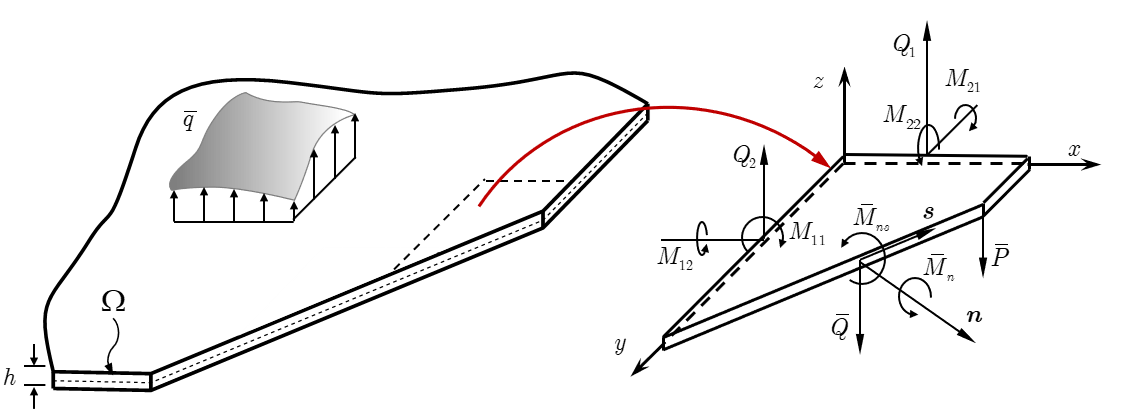
\includegraphics[scale=0.7]{figure/nomesh/plate.png}
    \caption{薄板运动学及边界条件}\label{plate}
\end{figure}
\noindent
其中式(\ref{P control equation})存在如下关系式:
\begin{subequations}
\begin{align}
\label{wn} &w_{,\pmb n}=w_{,\alpha}n_{\alpha}\\
\label{Qn} &Q_{\pmb n}=n_{\alpha}M_{\alpha\beta,\beta}\\
\label{Mn} &M_{\pmb{nn}}=M_{\alpha\beta}n_{\alpha}n_{\beta},M_{\pmb{ns}}=M_{\alpha\beta n_{\alpha}s_{\beta}},M_{\pmb{ns,s}}=M_{\alpha\beta,\gamma}s_{\alpha}n_{\beta}s_{\gamma}
\end{align}
\end{subequations}
式中$M_{\alpha\beta}$为矩量$\boldsymbol M$的弯曲和扭转分量,$\bar q$为垂直于薄板中面的分布荷载。$\Gamma_w$、$\Gamma_{\theta}$和$c_w$为本质边界条件,$\bar w$和$\bar \theta_n$分别为本质边界条件上给定的挠度和转角。
$\Gamma_V$、$\Gamma_M$和$c_P$为自然边界条件,$V_{\boldsymbol n}$、$M_{\boldsymbol{nn}}$和$P$为自然边界上的等效剪力、法向弯矩和薄板角上的集中荷载。$\pmb{n}=\{n_x,\; n_y\}^T$,$\pmb{s}=\{s_x,\; s_y\}^T$分别表示所在边界方向上的外法线方向和切方向的分量。
所有的边界条件都满足如下关系式:
\begin{equation}\label{PGeometric relationships}
    \begin{split}
        \Gamma=\Gamma_w\cup\Gamma_V\cup\Gamma_{\theta}\cup\Gamma_M,c=c_w\cup c_P\\
        \Gamma_w\cap\Gamma_V=\Gamma_{\theta}\cap\Gamma_M=c_w\cap c_P=\varnothing
    \end{split}
\end{equation}\par
当薄板为线弹性各同向性材料时,其本构关系为:
\begin{equation}
    \begin{split}\label{Malphabeta}
        M_{\alpha\beta}=D_{\alpha\beta\gamma\eta}\kappa_{\gamma\eta}=-D_{\alpha\beta\gamma\eta}w_{,\gamma\eta}
    \end{split}
\end{equation}
其中$\kappa_{\alpha\beta}$为曲率张量$\pmb{\kappa}$的分量,表达式如下:
\begin{equation}\label{kappa}
    \kappa_{\alpha\beta}=-w_{,\alpha\beta}
\end{equation}
式中$D_{\alpha \beta \gamma \eta}$为四阶弹性张量的分量,表达式如下:
\begin{equation}
    \begin{split}\label{Dalphabeta}
        D_{\alpha\beta\gamma\eta}=\bar D(\nu\delta_{\alpha\beta}\delta_{\gamma\eta}+\frac{1}{2}(1-\nu)(\delta_{\alpha\gamma}\delta_{\beta\eta}+\delta_{\alpha\gamma}\delta_{\beta\gamma}))
    \end{split}
\end{equation}
其中$\bar{D}$为抗弯刚度,抗弯刚度可由杨氏模量$E$、泊松比$\nu$和板厚$h$计算得到:
\begin{equation}\label{kangwangangdu}
    \begin{split}
    \bar D=\frac{Eh^3}{12(1-\nu^2)}
\end{split}
\end{equation}
\par
% 根据尺寸相关弹性\cite{Liu},将式(\ref{Qn})、(\ref{Mn})、(\ref{Malphabeta})、(\ref{Dalphabeta})代入式(\ref{P control equation})中可以得到自然边界上的法向弯矩$M_{\pmb{nn}}$、等效剪力$V_{\pmb{n}}$和薄板角上的集中荷载$P$的具体表达式:
% \begin{equation}
% \begin{split}\label{MVP}
%     \begin{cases}
%         M_{\pmb{nn}}=\mathcal{M}_{\alpha\beta}w_{,\alpha\beta}=-\bar{D}(\nu\delta_{\alpha\beta}+(1-\nu)n_{\alpha}n_{\beta})w_{,\alpha\beta}\\
%         V_{\pmb{n}}=\mathcal{V}_{\alpha\beta}w_{,\alpha\beta}=-\bar{D}(\frac{\partial}{\partial x_{\alpha}}n_{\beta}+(1-\nu)n_{\alpha}\frac{\partial}{\partial y_{\gamma}}s_{\alpha}n_{\beta}s_{\gamma})w_{,\alpha\beta}\\
%         P=\mathcal{P}_{\alpha\beta}w_{,\alpha\beta}=-[[(\bar{D}(1-\nu)n_{\alpha}s_{\beta})w_{,\alpha\beta}]]
%     \end{cases}
% \end{split}
% \end{equation}
% 其中:
% \begin{equation}
% \begin{split}\label{MVP1}
%     \begin{cases}
%  \mathcal{M}_{\alpha\beta}w_{,\alpha\beta}=-D_{\alpha\beta\gamma\eta}n_{\gamma}n_{\eta}=-\bar{D}(\nu\delta_{\alpha\beta}+(1-\nu)n_{\alpha}n_{\beta})\\
%   \mathcal{V}_{\alpha\beta}w_{,\alpha\beta}=-D_{\alpha\beta\gamma\eta}(n_{\gamma}\frac{\partial}{\partial x_{\eta}}+s_{\gamma}n_{\eta}s_{\xi}\frac{\partial}{\partial x_{\xi}})=-\bar{D}(\frac{\partial}{\partial x_{\alpha}}n_{\beta}+(1-\nu)n_{\alpha}\frac{\partial}{\partial y_{\gamma}}s_{\alpha}n_{\beta}s_{\gamma})\\
%  \mathcal{P}_{\alpha\beta}w_{,\alpha\beta}=-[[D_{\alpha\beta}n_{\gamma}s_{\eta}]]=-[[\bar{D}(1-\nu)n_{\alpha}s_{\beta}]]
%     \end{cases}
% \end{split}
% \end{equation}\par
根据最小势能原理,强形式(\ref{P control equation})所对应的的势能泛函表达式为:
\begin{equation}\label{Pshineng}
    \Pi(w)=\int_{\Omega}\frac{1}{2}\kappa_{,\alpha\beta}M_{\alpha\beta}d\Omega+\int_{\Gamma_M}\theta_{\pmb{n}}\bar{M}_{\pmb{nn}}d\Gamma
    -\int_{\Gamma_V}w\bar{V}_{\pmb{n}}d\Gamma-w\bar{P}\vert_{x\in c_P}+\int_{\Omega}w\bar{q}d\Omega
\end{equation}
对式(\ref{Pshineng})进行变分可以得到式(\ref{P control equation})的等效积分弱形式:
\begin{equation}\label{Pweakform}
\begin{split}
        \delta\Pi(w)&=\int_{\Omega}\delta\kappa_{,\alpha\beta}M_{\alpha\beta}d\Omega+\int_{\Gamma_M}\delta\theta_{\pmb{n}}\bar{M}_{\pmb{nn}}d\Gamma\\
        &-\int_{\Gamma_V}\delta w\bar{V}_{\pmb{n}}d\Gamma-\delta w\bar{P}\vert_{x\in c_P}+\int_{\Omega}\delta w\bar{q}d\Omega=0
\end{split}
\end{equation}\par
在伽辽金无网格法中,引入无网格近似离散挠度$w$及其变分$\delta w$,其近似函数$w^h$和$\delta w^h$的分量为:
\begin{equation}
\label{Pwuwangelisan}
    w_{\alpha\beta}^h(\pmb{x})=\sum_{I=1}^{N\!P}\Psi_I(\pmb{x})d_{\alpha\beta I},\quad \delta w_{\alpha\beta}^h(\pmb{x})=\sum_{I=1}^{N\!P}\Psi_I(\pmb{x})\delta d_{\alpha\beta I}
\end{equation}
式中$d_{\alpha\beta I}$、$\delta d_{\alpha\beta I}$分别为近似挠度分量$w_{\alpha\beta}^h$、$\delta w_{\alpha\beta}^h$在$w$处的节点系数。进一步将挠度表达式(\ref{Pwuwangelisan})代入曲率张量表达式(\ref{kappa})中可得:
\begin{equation}
\kappa_{\alpha\beta}=\sum_{I=1}^{N\!P}\Psi_{I,\alpha\beta}d_{\alpha\beta I}
% \pmb{B}_I(\pmb{x})= \left[\begin{matrix}\Psi_{I,xx}\\\Psi_{I,yy}\\2\Psi_{I,xy}\end{matrix}\right] 
\end{equation}
将式(\ref{wn})、(\ref{Malphabeta})和(\ref{Pwuwangelisan})代入到弱形式(\ref{Pweakform})中得到薄板问题伽辽金无网格法离散平衡控制方程:
\begin{equation}
     \pmb{K}\pmb{d}=\pmb{f}
\end{equation}
其中$\pmb{d}=\{d_{\alpha\beta I}\}$表示挠度节点系数向量,$\pmb{K}=\{\pmb{K}_{I\!J}\}$和$\pmb{f}=\{\pmb{f}_I\}$分别表示刚度矩阵和力向量,其分量具有表达式为:
\begin{subequations}\label{PKf}
\begin{align}
    \label{PKf1}\pmb K_{I\!J}&=\int_{\Omega}\pmb{B}^T_I\pmb{D}\pmb{B}_Jd\Omega\\
    \label{PKf2}\pmb f_I&=\int_{\Gamma_V}\Psi_I\bar{V}_{\pmb{n}}d\Gamma-\int_{\Gamma_M}\Psi_{I,\pmb{n}}\bar{M}_{\pmb{nn}}d\Gamma+\Psi_I\bar{P}\vert_{x\in c_P}+\int_{\Omega}\Psi_I\bar{q}d\Omega
\end{align}
\end{subequations}
式中$\pmb{D}$为四阶弹性张量,$\pmb{B}_I$为形函数梯度矩阵,其形函数梯度矩阵具有如下表达式:
\begin{equation}
\pmb{B}_I(\pmb{x})= \left[\begin{matrix}\Psi_{I,xx}\\\Psi_{I,yy}\\2\Psi_{I,xy}\end{matrix}\right] 
\end{equation}
\section{小结}
本章首先对再生核无网格近似理论进行了系统分析,讨论了再生核无网格形函数的一致性条件。再生核无网格法是一种用于求解偏微分方程的数值积分方法,
是指通过离散点之间的相对位置关系来进行近似。接下来以弹性力学问题和薄板问题为例,详细介绍了伽辽金无网格法在这两类问题上的离散平衡控制方程。
在弹性力学问题中,伽辽金无网格法利用再生核无网格形函数近似位移场,在薄板问题中,伽辽金无网格法同样采用再生核无网格形函数近似挠度场。
与传统有限元法不同,再生核无网格形函数通常不具备插值性,因此需要采用适当的方法进行施加强制边界条件。
